\pagestyle{mystyle}

\part{空间任务挑战与发展展望}

\renewcommand{\parttitle}{空间任务挑战与发展展望}

\chapter{空间引力波探测任务的数据挑战}

地面引力波探测器（LIGO、Virgo、KAGRA）的成功，开创了引力波天文学的新纪元。然而，地面探测器受限于地球尺度和地震噪声，灵敏频段通常在 10 Hz 以上，无法探测更丰富的低频引力波源。空间引力波探测器——欧洲的 LISA（Laser Interferometer Space Antenna）、中国的太极（Taiji）和天琴（TianQin）——将把探测窗口延伸至毫赫兹频段，开辟一个全新的引力波宇宙窗口。

然而，这一频段的丰富性也带来了新的数据分析挑战。王赫等人~\cite{wang2024challenges} 的综述系统梳理了这些挑战：数百万个信号同时叠加、非稳态仪器噪声、极端质量比旋近的高维参数空间，以及全局拟合的巨大计算代价。Du 等人~\cite{du2026taiji} 的受邀综述进一步指出，从理想化模拟到真实探测管道，太极任务面临的挑战比早期简化模型更复杂。本章以太极任务为主线，系统分析这些挑战的物理根源，并讨论人工智能方法在各个环节可能提供的解决路径。

\section{空间引力波探测器的科学目标与数据特征}

太极计划由中国科学院主导，三颗卫星组成等边三角形星座，臂长约 300 万公里，采用与地球保持约 $20^\circ$ 角距离的日心轨道方案。其主要科学目标涵盖四类引力波源：

\textbf{大质量双黑洞并合}（MBHBs，$10^5$--$10^8\,M_\odot$）：星系并合的产物，在空间引力波探测窗口中可形成高信噪比信号，部分事件可能伴随电磁辐射，是多信使天文学的重要目标。

\textbf{极端质量比旋入}（EMRIs）：恒星质量致密天体螺旋并入超大质量黑洞，在并合前经历超过 $10^5$ 圈轨道，携带极丰富的强引力场信息，是检验广义相对论的精密探针。

\textbf{银河系双星}（Galactic Binaries）：数百万个双白矮星系统同时辐射引力波，在低频段形成“混淆噪声”背景，既是科学目标，也是数据分析的主要干扰源。

\textbf{随机引力波背景}（SGWB）：早期宇宙相变、宇宙弦等过程产生的随机引力波叠加，携带宇宙学信息。

与地面探测器相比，空间引力波数据的核心特征是\textbf{信号密度极高}：在任意时刻，探测器同时接收来自数百万个银河系双星、数十个 EMRI 以及偶发的 MBHB 并合信号，许多信号在频域严重叠加。这使得逐一独立分析单个信号的传统流程难以直接适用。

\subsection{太极的轨道与技术参数}

太极计划的技术方案在多个关键指标上与欧洲的LISA形成互补关系。在轨道设计上，太极三颗卫星绕日运行，星座中心与地球保持约$20^\circ$角距离；LISA同样采用日心轨道并与地球保持数千万公里量级的相位差。两者若在时间上形成重叠观测，其轨道位置和臂长差异将带来不同的方向图响应，从而提高联合观测对天空位置、极化和距离参数的约束能力。

在核心技术指标上，太极方案通常以较长臂长和较低位移噪声为设计目标。代表性参数包括位移噪声目标约 $1\,\mathrm{pm}/\sqrt{\mathrm{Hz}}$、加速度噪声目标约 $3\times10^{-15}\,\mathrm{m/s^2}/\sqrt{\mathrm{Hz}}$、激光链路长度约3Gm。与臂长约250万公里的LISA相比，太极在部分中低频段可能具有不同的灵敏度侧重，尤其有利于探测质量较大的MBHB系统；具体灵敏度仍取决于最终工程指标和噪声预算。

太极与LISA在科学目标上高度互补。两者频率覆盖范围相近（均主要面向毫赫兹频段），但由于臂长、轨道和噪声预算的差异，对具体质量和红移区间的灵敏度各有侧重。LISA已完成Pathfinder任务的关键技术验证，并于2024年获得ESA正式采纳；太极正在通过太极一号（2019年）和后续技术验证任务逐步积累技术储备，目标发射时间通常设定在2030年代。

\subsection{天琴的近地轨道方案及其特点}

天琴计划由中山大学主导，采用与太极/LISA根本不同的近地轨道方案。三颗卫星绕地球运行，轨道高度约10万公里，臂长约17万公里——仅为LISA/太极的约7\%。这一设计的出发点是充分利用近地轨道的工程优势：地球引力场在近地范围内测量精度更高，轨道维持控制更为成熟，与地面测控站的通信窗口更为充裕，整体任务风险低于日心轨道方案。

然而，臂长的大幅缩短对科学能力产生了深刻影响。天琴的峰值灵敏度频段约在 $10^{-3}$--$10^{-1}$ Hz，与太极/LISA有一定重叠，但在低频端（$<10^{-3}$ Hz）的灵敏度因臂长受限而下降。天琴的科学重点因此集中在几类特定源：已知超紧凑双星和银河系双星、大质量双黑洞的并合晚期阶段、部分EMRI候选以及基础物理检验。特别地，天琴对RX J0806.3+1527等已知超紧凑双星系统有望实现高精度观测，这类“验证源”的探测将为天琴提供宝贵的数据分析标定机会。

从数据分析角度，天琴的近地轨道带来一个额外复杂性：地球重力场的不均匀性会向卫星引入额外的力学噪声，需要更精密的无拖曳控制技术。但同时，近地轨道也使得天琴能够与地基引力波探测器形成独特的联合观测配置——对于某些在两者频段重叠区间（约 $10^{-2}$--$1$ Hz）的信号，天琴与LIGO/Einstein Telescope的联合分析可以实现更好的参数估计。

\subsection{三任务联合观测的科学增益}

太极、LISA和天琴三个任务若能形成时间重叠的联合观测，将带来超过单任务分析的科学增益，这一增益在多个维度均有体现。

在天空定位精度上，太极与LISA的联合观测相当于构建了一个由两套日心星座组成的空间干涉网络。由于两者在轨道相位、臂长和方向图响应上存在差异，联合分析有望打破单任务天空位置、倾角和距离之间的部分简并。对于MBHB系统，单任务的天空定位精度通常可从数十到数百平方度不等（取决于信号持续时间、SNR和并合前预警时间），而太极+LISA的联合分析在有利情形下可将定位面积显著缩小，使并合前宿主星系候选筛选更为可行。天琴加入后，三任务联合分析可能进一步提高定位能力，但实际精度仍取决于源参数、任务重叠时间和噪声状态。

在参数估计精度上，联合观测的增益同样重要。对MBHB系统，联合分析可改善距离、天空位置和倾角等外禀参数的联合约束，对标准汽笛宇宙学具有重要价值。对于EMRI，不同探测器方向图有望帮助打破轨道倾角、偏心率、天空位置等参数简并，使参数估计精度获得不同程度的提升。更重要的是，不同探测器对同一信号的独立测量提供了交叉验证手段，有助于识别和控制系统误差。

在探测灵敏度上，三任务联合分析还可以降低误报率。对于弱信号（SNR接近检测阈值），单任务的信号候选体往往难以区分真实信号与噪声涨落，而要求多任务同时确认则可以将误报概率降低数个量级。这对于随机引力波背景的探测尤为关键——单任务探测背景信号需要长期积分，而多任务的相关分析可以更快速地达到所需的统计显著性。

\subsection{各类源的预期探测率与参数范围}

基于当前的天体物理模型，各类引力波源的预期探测参数有以下估算。对于MBHB，预期年探测率约10--100个，质量范围 $10^4$--$10^8\,M_\odot$，红移可达 $z\sim10$，对应宇宙大尺度结构形成的早期阶段。高红移MBHB的探测对理解超大质量黑洞的种子形成机制具有关键意义——目前关于超大质量黑洞形成是否通过“种子黑洞”（$10^3$--$10^4\,M_\odot$）的逐步并合还是直接塌缩（$>10^5\,M_\odot$）仍存在争议，MBHB探测率的红移分布可以直接约束这两种模型。

对于EMRI，预期年探测率跨越更大范围，约10--1000个，具体数值对星系核星团密度、俘获率和探测阈值等假设高度敏感。EMRI的轨道参数（偏心率、轨道倾角）在螺旋并入过程中经历复杂的进动演化，使得波形对Kerr时空的几何结构极为敏感。在有利信噪比和波形系统误差可控的条件下，单个EMRI事件有望将超大质量黑洞质量和自旋测量到极高精度。这一“强引力场精密测量”能力使EMRI成为检验广义相对论和无毛定理的重要工具之一。

银河系双白矮星背景预计包含约 $10^7$ 个双星系统同时辐射引力波，其中在 $10^{-3}$ Hz以上频段可分辨的约有 $10^4$ 个。这些可分辨双星将构成“引力波星图”——对银河系双星种群的统计研究，可以约束双星演化通道（特别是公共包层演化阶段）和银河系化学演化历史。随机引力波背景方面，预期在 $10^{-3}$--$10^{-2}$ Hz频段可能探测到原初引力波或宇宙相变背景，但具体振幅对早期宇宙模型高度依赖，探测有一定不确定性。

\begin{figure}[htbp]
\centering
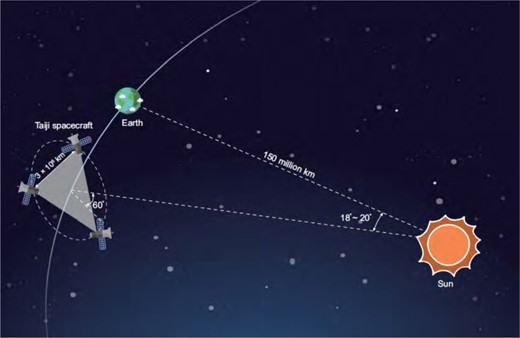
\includegraphics[width=0.86\textwidth]{figures/PTEP2021_Taiji_fig1.jpeg}
\caption{太极（Taiji）空间引力波探测器星座示意图。太极三颗航天器构成臂长约 $3\times10^6\,\mathrm{km}$ 的近似等边三角形星座，星座中心沿日心轨道运行，并与地球保持约 $18^\circ$--$20^\circ$ 的角距离。该轨道构型使太极在毫赫兹频段获得长期稳定的空间干涉基线，也为与 LISA 等日心轨道任务开展联合观测提供了方向图互补性。图片引自 Luo 等~\cite{Luo2021Taiji_PTEP} 的 Figure 1。}
\label{fig:taiji_constellation}
\end{figure}

\section{全局拟合：空间引力波数据分析的核心难题}

全局拟合（Global Fit）是空间引力波数据分析的重要目标：同时对探测器数据中大量重叠信号源进行联合参数估计。其必要性来自信号的相互耦合——单个信号的参数估计会受到其他信号的干扰，联合分析是控制这类系统误差的关键途径。

全局拟合的计算挑战极为严峻。参数空间维度可达到 $10^5$--$10^7$ 量级，具体取决于可分辨银河系双星数量、是否显式建模弱源混淆背景、EMRI数量以及SGWB参数化方式。传统 MCMC 方法难以直接用于如此高维且强相关的参数空间，即便采用先进的嵌套采样算法，完整全局拟合也可能超出现实任务预算。

当前最接近实用的全局拟合方案多采用迭代减除或分块联合拟合策略：首先识别并减除最强或最易分离的信号，然后在残差数据上继续搜索和更新其他源，如此迭代直至主要可分辨信号被提取。这一策略的关键假设是信号强度和频域结构存在可利用的层级，以及每步减除的精度足够高以避免残差污染后续步骤。AI 方法在每个迭代步骤中的快速搜索和参数估计能力，是使这一策略在实践中可行的重要技术支撑。

人工智能方法在全局拟合中的角色是分层的：快速搜索方法（第5章）提供强信号的初始定位，SBI 方法（第6章）对各类源进行快速参数估计，去噪方法（第7章）处理非稳态噪声，最终由全局拟合框架整合这些中间结果。这一分层架构使人工智能方法不再只是单点工具，而成为空间任务数据处理基础设施的一部分。

\subsection{全局拟合的数学框架}

全局拟合的核心是对联合后验分布的估计。设探测器数据为 $d$，探测器中同时存在 $K$ 个信号源，第 $k$ 个信号源的参数向量为 $\theta_k$，则全局后验分布为：
\begin{equation}
p(\{\theta_k\}_{k=1}^K | d) \propto p(d|\{\theta_k\}) \prod_{k=1}^K p(\theta_k),
\end{equation}
其中 $p(\theta_k)$ 是各信号源参数的先验分布，$p(d|\{\theta_k\})$ 是联合似然函数。由于大量信号在频域叠加，联合似然函数通常不能简单分解为各信号似然的乘积——许多频率bin同时携带多个信号的贡献，使得对单一信号源的分析需要同时考虑其他强信号、混淆背景和噪声模型。

在高斯噪声假设下，联合似然函数的对数为：
\begin{equation}
\ln p(d|\{\theta_k\}) = -\frac{1}{2} \left\langle d - \sum_k h(\theta_k) \,\bigg|\, d - \sum_k h(\theta_k) \right\rangle,
\end{equation}
其中 $h(\theta_k)$ 是第 $k$ 个信号源在探测器中产生的应变，内积 $\langle \cdot | \cdot \rangle$ 按噪声功率谱密度加权。由于参数总维度 $\sum_k \dim(\theta_k)$ 可达 $10^5$--$10^7$ 量级，直接对联合后验进行逐点采样在当前计算预算下难以承担。

当前代表性的全局拟合实现多采用分块-迭代策略：将 $K$ 个信号源按类型分组（MBHB组、EMRI组、银河系双星组、背景组），在每个迭代步骤中固定或边缘化其他组的近似参数，对当前组进行贝叶斯推断，然后更新当前组的参数后继续迭代。这一策略将高维联合优化分解为一系列低维子问题，但代价是收敛速度较慢且依赖良好的初始化。

GLASS、BALROG 等框架是当前空间引力波全局拟合研究中的代表性实现。它们通常采用迭代残差减除、贝叶斯模型选择、多模态采样或分块优化等技术，在LISA数据挑战（LDC）等模拟数据上验证了处理复杂多源场景的可行性。不同框架在计算效率、模型完备性和后验精度之间有不同取舍，距离完整任务规模的在线全局拟合仍需进一步发展。

\subsection{AI在全局拟合中的分层架构}

\begin{figure}[htbp]
\centering
\resizebox{0.96\textwidth}{!}{%
\begin{tikzpicture}[
  font=\small,
  band/.style={draw, rounded corners=5pt, minimum width=12.2cm, minimum height=1.85cm,
               align=left, inner sep=5pt},
  l0/.style={band, fill=gray!10, draw=gray!50},
  l1/.style={band, fill=blue!7, draw=blue!45},
  l2/.style={band, fill=green!7, draw=green!45},
  l3/.style={band, fill=orange!8, draw=orange!55},
  method/.style={draw, rounded corners=2pt, minimum width=3.35cm, minimum height=0.68cm,
                 text centered, align=center, font=\scriptsize, fill=white},
  layerlabel/.style={font=\small, align=left},
  arr/.style={-Stealth, thick, gray!60},
]
\node[l0] (lay0) at (0,0) {};
\node[l1, below=4mm of lay0] (lay1) {};
\node[l2, below=4mm of lay1] (lay2) {};
\node[l3, below=4mm of lay2] (lay3) {};

\node[layerlabel, anchor=north west] at ([xshift=4mm,yshift=-3mm]lay0.north west)
  {第零层：快速搜索层（毫秒--秒级）};
\node[layerlabel, anchor=north west] at ([xshift=4mm,yshift=-3mm]lay1.north west)
  {第一层：参数估计层（秒--分钟级）};
\node[layerlabel, anchor=north west] at ([xshift=4mm,yshift=-3mm]lay2.north west)
  {第二层：全局融合层（天--周级）};
\node[layerlabel, anchor=north west] at ([xshift=4mm,yshift=-3mm]lay3.north west)
  {第三层：验证层（PP图、覆盖率检验）};

\node[method] (m01) at ([xshift=-3.9cm,yshift=-0.45cm]lay0.center) {MBHB快速搜索\\Ruan等，秒级};
\node[method] (m02) at ([yshift=-0.45cm]lay0.center) {EMRI两层CNN\\Yun等，分钟级};
\node[method] (m03) at ([xshift=3.9cm,yshift=-0.45cm]lay0.center) {全源统一检测\\Zhao等，模拟};

\node[method] (m11) at ([xshift=-3.9cm,yshift=-0.45cm]lay1.center) {归一化流/CNF\\MBHB（秒级）};
\node[method] (m12) at ([yshift=-0.45cm]lay1.center) {CNF-EMRI\\17维（分钟级）};
\node[method] (m13) at ([xshift=3.9cm,yshift=-0.45cm]lay1.center) {批量参数估计\\银河系双星（ms级）};

\node[method, minimum width=4.2cm] (m21) at ([xshift=-2.2cm,yshift=-0.45cm]lay2.center)
  {全局拟合优化器\\分块联合推断};
\node[method, minimum width=4.2cm] (m22) at ([xshift=2.2cm,yshift=-0.45cm]lay2.center)
  {残差信号更新\\迭代减除与回填};

\node[method, minimum width=4.2cm] (m31) at ([xshift=-2.2cm,yshift=-0.45cm]lay3.center)
  {统计校准\\PP图与覆盖率};
\node[method, minimum width=4.2cm] (m32) at ([xshift=2.2cm,yshift=-0.45cm]lay3.center)
  {物理审查\\异常事件复核};

\draw[arr] (lay0.south) -- (lay1.north);
\draw[arr] (lay1.south) -- (lay2.north);
\draw[arr] (lay2.south) -- (lay3.north);
\end{tikzpicture}}
\caption{空间引力波数据分析的分层人工智能架构示意图。第零层（快速搜索）在秒至分钟级内完成数据流的信号普查，提供参数空间初始定位；第一层（参数估计）对各类源进行快速近似或精细参数估计；第二层（全局融合）以第一层结果为初始值运行全局拟合；第三层（验证）通过PP图和覆盖率检验等工具评估结果的统计可靠性。图中时间尺度为基于现有代表性研究的任务级估计，并非完整任务流水线的正式性能指标；相关方法背景依据文献~\cite{ruan2023mbhb,zhao2023spacegw,liang2026sbireview,wang2024challenges,du2026taiji}综合改绘。}
\label{fig:global_fit_layers}
\end{figure}

当前主流的解决思路是构建分层的人工智能辅助架构，将全局拟合分解为多个计算上可行的子问题，由不同的人工智能组件分别处理，最后通过全局优化器整合结果。

第零层（快速搜索层）负责对数据中各类信号的初步普查。Ruan等的MBHB快速搜索在数秒内完成对一年模拟数据的扫描；Yun等的EMRI两层CNN探测器在分钟级时间内完成对EMRI候选体的普查；Zhao等的全源统一检测网络在所采用的模拟设置中同时标记多类信号候选。这一层的输出是各类信号候选体的初步位置（在参数空间中的粗定位），为后续精确推断提供初始化信息，减少从宽先验出发的低效采样。

第一层（参数估计层）对各类源的参数进行快速近似或精细估计。归一化流和CNF方法可对MBHB候选体给出约15维参数后验（秒至分钟级）；CNF方法对EMRI候选体探索17维参数后验估计；简单参数化方法可对银河系双星给出低维参数估计（毫秒级，适应大规模批量处理）。这一层的输出是各信号源的近似参数后验分布，作为第二层全局融合的输入。

第二层（全局融合层）将第一层结果作为初始值或提议分布，运行全局拟合算法。由于第一层已经提供了较好的初始参数估计，全局拟合所需的迭代次数有望减少，计算代价可能从月级量级压缩至天至周级量级。全局融合层的输出是联合后验分布的近似，用于计算主要可分辨信号源参数的最终估计和不确定度。

第三层（验证层）对第二层输出进行统计一致性检验：PP图检验SBI输出的后验分布是否经过校准，覆盖率检验确认可信区间的统计意义，并对异常事件（如显著偏离GR预言的信号）开展专项分析。这一层的存在是全局拟合结果能够获得科学界信任的必要条件。

\subsection{迭代减除的误差积累与AI精度要求}

迭代减除策略的可行性依赖于每步减除的精度足够高，使得残差中的信号残留不会对后续步骤造成显著污染。量化分析这一要求，可以给出AI方法精度的硬性门槛。

设每步参数估计的系统误差为 $\epsilon$（定义为参数估计偏差与真值之比），则该步减除后，残差中保留的信号功率约为 $\epsilon^2$ 倍的原始信号功率。对于有 $N$ 个可分辨银河系双星的迭代减除，若每步精度 $\epsilon$，则经过 $N$ 步后，残差中所有双星的信号残留叠加的总功率约为 $N\epsilon^2$ 倍的平均信号功率。当 $N\epsilon^2 \sim 1$ 时，残差噪声地板与单个双星信号相当，后续的EMRI等弱信号分析将受到严重干扰。

对于 $N\sim10^4$（可分辨银河系双星数量的保守估计），这一简单估算给出 $\epsilon < 1/\sqrt{N} \approx 0.01$ 的量级要求，即每步参数估计的系统误差需要接近百分之一量级。真实管道中的要求会随信号强度分布、频率重叠程度和误差相关性而变化，但这一估算说明：SBI方法的系统误差（由训练集偏差、网络容量限制等引起）需要被严格校准，才可能支撑迭代减除的稳定运行。进一步压缩并量化系统误差，是全局拟合从概念验证走向实际应用的关键技术挑战。

\section{主要波源类型的人工智能分析方法}

\subsection{大质量双黑洞：从快速搜索到精确参数估计}

MBHB 并合是空间引力波探测器最强的信号源，其低延迟探测对多信使天文学至关重要。Ruan 等人~\cite{ruan2023mbhb} 开发的深度学习快速搜索方法能够在\textbf{数秒量级}处理一年的 LISA 模拟数据；在所采用的测试集中，该方法识别了注入的 MBHB 并合事件，并未报告误报。需要强调的是，这一结果来自特定模拟数据集和评估条件，真实任务中的误报率还需结合噪声非平稳性、数据质量标记和统计显著性评估进一步验证。即便如此，其计算效率的量级优势仍使其成为全局拟合分析的有力初始化工具。

在参数估计层面，Du、Liang、Wang 等人~\cite{du2024normflow} 将归一化流方法应用于太极任务的 MBHB 参数估计，处理了太极特有的时变响应函数和混淆噪声背景，实现比传统方法快几个数量级的推断速度。Liang 等人~\cite{liang2024cnfmbhb} 进一步引入连续归一化流（CNF）和流匹配技术，在精度和速度上均有提升。Sun 等人~\cite{sun2025cvae} 的混合推断方案（CVAE + 贝叶斯采样）在三探测器（太极 + LISA + 天琴）联合观测场景下，将采样时间压缩至原来的 14.0\%，同时维持贝叶斯精度。

在具体方法实现上，Ruan等的深度学习快速搜索使用ResNet作为骨干网络，输入为TDI（时间延迟干涉）AET数据通道的时频表示。网络在LDC Radler数据集（包含若干注入MBHB事件的1年模拟数据）上训练和测试，在该设置中成功识别注入事件且未报告误报，单次处理时间约为秒级。相比于传统模板搜索方法，这一计算优势使得MBHB的近实时监测成为可能，对于捕捉电磁对应体具有重要意义。

Du等的归一化流参数估计在对数总质量、质量比、自旋、天空位置、距离、倾角、极化角和并合时刻等约15个参数上给出后验估计。特别值得注意的是，太极的时变响应函数会使天空位置后验呈现多模态结构（一年运动过程中，探测器对同一天空位置的敏感性随时间变化，导致存在多个似然极大值），而归一化流方法的生成建模能力有助于处理这种多模态性。Liang等的CNF方法（基于流匹配技术）进一步改善了多模态后验的建模，在天空位置参数的覆盖率检验中表现出较好校准性。

\subsection{极端质量比旋入：高维参数空间的突破}

EMRI 是空间引力波数据分析中最困难的问题之一。其 17 维参数空间、强参数简并（多极大值似然函数）、以及较高的波形计算代价，使直接传统 MCMC 方法在现实计算预算下面临严峻挑战。

Yun 等人~\cite{yun2024emri} 提出的两层 CNN 方法在 SNR 50--100 的模拟范围内实现了 96.9\% 的 EMRI 探测真正率，并在测试设置中给出超大质量黑洞质量和自旋的高精度估计，为后续参数估计压缩搜索空间。Liang 等人~\cite{liang2024cnfemri} 将连续归一化流应用于 EMRI 参数估计，在 17 维参数空间中展示了比传统采样快几个数量级、且在模拟测试中通过校准检验的推断能力，是机器学习方法进入这一高难度问题的重要进展。

Yun等的两层CNN方法针对EMRI探测的特殊困难进行了专门设计。EMRI信号在频域表现为密集的谐波梳状结构，每个谐波的频率随时间缓慢演化（频率漂移量级取决于源参数），与银河系双星的近单频信号有本质区别。第一层CNN输入为TDI AET通道数据的时频谱图，通过多尺度卷积捕获EMRI谐波的特征模式，输出为“EMRI候选”或“非EMRI”的二分类决策。第二层CNN对第一层确认的候选体进行精细特征提取，直接估计超大质量黑洞的质量和自旋——这两个参数决定了Kerr时空的主要几何特征，是EMRI轨道频率结构的主要决定因素。通过预先估计这两个参数，后续精确参数估计的搜索空间可从17维压缩至约15维，从而降低计算代价。

Liang等的CNF-EMRI工作是机器学习方法在空间引力波数据分析中值得重视的成果，其意义超越了单纯的技术加速。在方法论层面，它表明SBI方法有能力处理引力波数据分析中高度困难的参数估计问题——17维强简并参数空间中的多极大值后验分布——而传统MCMC方法对此类问题的收敛时间可能达到多年量级。在科学意义层面，更高效的EMRI参数估计将支持太极/LISA实现其旗舰科学目标——对超大质量黑洞周围Kerr时空的精密测绘，并为广义相对论和黑洞无毛定理的强场检验提供关键数据分析工具。在方法论推广层面，CNF在EMRI这一高难度问题上的成功，说明SBI方法有潜力扩展到更广泛的高维强简并推断场景，但其适用范围仍需要在更多物理模型、噪声条件和先验设定下系统检验。

Liang等的CNF-EMRI方法是当前EMRI参数估计中具有代表性的机器学习实现。训练集由FastEMRIWaveforms（FEW）生成的约50万条EMRI波形（覆盖17维参数空间）组成，FEW通过快速波形生成技术显著降低了单条波形的生成时间。网络架构为条件归一化流，以TDI AET三通道的频域表示为条件输入，输出17维参数的联合后验分布。在独立测试集上，17个参数的PP图在统计误差内通过一致性检验，表明后验分布在该模拟设置下具有良好的校准性。推断时间达到秒级或亚秒级（GPU加速），较传统采样方法实现了数量级加速。

\subsection{全源类型统一检测}

Zhao 等人~\cite{zhao2023spacegw} 提出的多阶段自注意力深度神经网络，在所采用的模拟设置下探索了对多类空间引力波源（银河系双星、MBHB、EMRI、随机背景）的统一检测与提取；在 SNR = 50、误报率 1\% 的条件下，各类源检测率达到较高水平。这一统一框架的意义在于：它减少了为每类源单独开发和维护专用算法的工程复杂性，为全局拟合管道提供了统一信号检测前端的可能方案。

多阶段自注意力架构的核心设计思想是：不同类型的引力波信号具有不同的时频特征模式，但都可以在足够宽广的特征空间中被统一表示。第一阶段使用多尺度卷积提取局部时频特征（适合捕获银河系双星的单频模式和EMRI的谐波梳结构）；第二阶段使用Transformer自注意力机制捕获长程时序相关性（适合追踪MBHB长达数月的旋入演化）；第三阶段使用多头输出头（multi-head output）同时对四类源给出检测决策。

在SNR = 50的模拟条件下，MBHB、EMRI和双白矮星等源的检测率均达到较高水平，随机背景振幅估计也表现出一定精度；在SNR较低的样本上，检测率有所下降但仍保持可用水平。这一统一检测框架在实际全局拟合管道中可以作为数据预处理的第一道关口，快速筛选出各类信号候选体，为后续专用参数估计方法提供输入。其真实任务性能仍需在更复杂噪声、源重叠和不完整训练分布下进一步验证。

\section{非稳态噪声：从理想模拟到真实管道}

早期空间引力波数据分析研究大多基于理想化的平稳高斯噪声假设。然而，真实的空间探测器在运行中不可避免地产生各种非稳态噪声，这些噪声在地面测试中难以完全预测和模拟。

Xu 等人~\cite{xu2024nonstationarty} 系统研究了三类可预见的非稳态噪声：数据间隙（例行维护或意外中断导致的数据缺失）、暂态噪声（仪器或环境扰动产生的短时高幅度脉冲）、以及时变噪声自相关（噪声功率谱密度的缓慢漂移）。针对这三类噪声及其混合情形，该工作开发的深度学习模型在保持理想场景性能的同时，展示了显著的非稳态适应性。

Du 等人~\cite{du2026taiji} 的受邀综述进一步指出，从理想化的 LISA 数据挑战（LDC）场景到太极真实探测管道，数据分析面临的挑战远比预期复杂：高保真探测器响应仿真、轨道动力学效应、时间延迟干涉（TDI）的精确实现，以及多种噪声源的联合建模，都需要系统性的方法论突破。

\subsection{太极的噪声模型与TDI原理}

太极的噪声模型由三类主要成分构成，各自在不同频段主导探测器的灵敏度极限。

第一类是加速度噪声（acceleration noise），来源于残余气体分子碰撞、宇宙线打击、热辐射压力涨落等对检验质量的随机力扰动。其功率谱密度为：
\begin{equation}
S_a(f) = \left(3\times10^{-15}\right)^2 \left[1 + \left(\frac{4\times10^{-4}\,\mathrm{Hz}}{f}\right)^2\right] \,\mathrm{m^2\,s^{-4}\,Hz^{-1}},
\end{equation}
在低频段（$f < 4\times10^{-4}$ Hz）随 $f^{-2}$ 增长，是低频灵敏度的主要限制因素。

第二类是光学路程噪声（optical path noise），来源于激光相位噪声残余、光子散粒噪声、望远镜热形变等。其功率谱密度约为：
\begin{equation}
S_\mathrm{opt}(f) \approx \left(1\times10^{-12}\right)^2 \,\mathrm{m^2\,Hz^{-1}},
\end{equation}
在高频段（$f > 10^{-2}$ Hz）近似为白噪声，是高频灵敏度的主要限制因素。

第三类是激光频率噪声，其量级约为 $10^9$ Hz/$\sqrt{\mathrm{Hz}}$，比引力波信号（等效位移噪声约 $10^{-12}$ m/$\sqrt{\mathrm{Hz}}$）大约12个量级。如此巨大的激光频率噪声必须通过时间延迟干涉（TDI）技术消除，才能使引力波信号从噪声中显现。

TDI的工作原理是通过延迟各臂的激光信号并进行线性组合，在代数上抑制激光频率噪声。以最简单的Michelson X通道为例，其构造可示意为：
\begin{equation}
X = (D_{31}D_{13} - 1)h_1 + (D_{13} - D_{31})h_2 + \cdots,
\end{equation}
其中 $D_{ij}$ 表示沿臂 $ij$ 方向的时间延迟算符，$h_i$ 表示第 $i$ 颗卫星上的激光相位测量。当臂长近似恒定时，激光频率噪声可在一阶TDI组合中高度相消；当臂长随时间变化时，需要使用第二代TDI（TDI 2.0）处理时变臂长效应。实际数据处理中，亚采样延迟通过Lagrange插值或sinc插值实现，插值精度直接影响TDI的激光噪声抑制效果。

TDI生成的A、E、T三个正交通道（由X、Y、Z通道的线性组合构成）具有不同的方向图响应：A和E通道对引力波信号敏感，T通道在低频段对引力波不敏感，可用于监测仪器噪声。这三个通道的联合分析是空间引力波数据处理的标准输入格式。

\subsection{三类非稳态噪声的物理机制与影响}

数据间隙是空间引力波探测器运行中需要重点考虑的非稳态数据质量问题。其来源包括：例行维护操作（激光重新锁定、推进器点火调轨）、意外中断（宇宙线打击导致的仪器复位）、以及数据传输中断。典型的数据间隙持续时间可能从数秒到数小时不等，发生率需由实际任务运行状态和地面测控策略确定。

数据间隙对TDI的影响具有特殊性：由于TDI利用延迟相消，单臂数据间隙会通过延迟算符传播，导致TDI输出的多个时间点同时受影响。具体地，若某臂在时刻 $t_0$ 发生持续 $\Delta t$ 的数据间隙，则TDI X通道在 $t_0$、$t_0 + L/c$、$t_0 + 2L/c$ 等多个时刻均受到影响（$L$ 为臂长，$c$ 为光速），形成“扩散”的噪声超出。这一传播效应使得数据间隙的影响范围远大于间隙本身的持续时间，对后续信号分析造成更广泛的干扰。

暂态噪声（glitch）在太空环境中的来源可能包括宇宙线打击、激光锁定失调、推进器动作和热控扰动等。高能粒子穿过检验质量时，可能通过电荷沉积或动量传递引发短时扰动；太阳活动周期也会影响带电粒子环境。由于具体发生率和振幅分布依赖探测器设计、轨道环境和在轨控制策略，相关模型应在技术验证任务和主任务早期数据中持续标定。

时变噪声自相关（time-varying noise PSD）可能来源于探测器热环境、激光链路状态、检验质量带电状态和太阳活动等因素的缓慢变化。卫星热控系统虽然维持激光器和光学平台的温度稳定，但微小温度涨落仍可能导致激光功率、光学路程和加速度噪声的缓慢漂移。此外，太阳耀斑、日冕物质抛射等事件会影响卫星热环境和带电粒子环境，导致噪声特性的突变。

Xu等鲁棒模型的关键设计是在训练集中系统性地引入各类非稳态噪声的模拟样本，使网络学习对噪声类型变化较不敏感的表示。在理想噪声、数据间隙、glitch以及混合非稳态噪声等测试情形中，鲁棒模型相对于只在理想噪声上训练的基线表现出更稳定的重叠度。这一结果表明，通过训练集的系统性扩充，可以在受控模拟条件下显著提升模型对复杂运行条件的适应能力；但其在真实在轨噪声中的表现仍需要后续数据验证。

\section{高保真仿真与现实探测管道的构建}

空间引力波数据分析算法的开发和验证，依赖于高保真的模拟数据。Du 等人~\cite{du2026taiji} 的综述系统梳理了太极高保真仿真的关键要素：

\textbf{探测器响应仿真}：太极星座的轨道运动导致探测器响应函数随时间变化（一年周期），需要精确的轨道动力学模型和时间延迟干涉（TDI）实现。早期工作（Du、Liang、Wang 等~\cite{du2024normflow}）已揭示这一时变响应在参数估计中引入的额外多模态结构。

\textbf{波源模型的完备性}：高保真仿真需要覆盖主要预期波源类型，包括银河系双星种群模型、MBHB 波形、EMRI 的 Kerr 时空轨道演化，以及各类随机背景的功率谱模型。

\textbf{噪声模型的真实性}：从理想高斯噪声到包含非稳态成分的真实噪声，是算法从实验室走向实际应用的关键一步。Xu 等人~\cite{xu2024nonstationarty} 的工作为这一过渡提供了方法论基础。

\textbf{多任务协同}：太极、LISA、天琴三个任务若能形成重叠观测，将有望提升参数估计精度（Sun 等~\cite{sun2025cvae} 在三探测器场景下的验证）和天空定位能力。跨任务算法的共享与优化，是降低整体研发成本的重要方向。

空间引力波数据分析的最终目标，是构建一个能够在任务运行期间持续、自动、可靠地处理海量数据的完整管道。这一管道需要将本书前述各章的方法——信号识别（第5章）、参数估计（第6章）、去噪（第7章）、算法自动发现（第8章）、物理-数据融合（第9章）——有机整合，形成一个既高效又可靠的科学数据处理系统。AI 方法在这一系统中不只是单点性能优化，而是提高完整管道计算可行性的重要使能技术。

高保真仿真基础设施的建设不仅服务于算法开发和测试，还在科学验证中发挥关键作用。太极任务发射后，高保真仿真器可用于校准在轨探测到的信号：通过将观测数据与高保真模拟预测对比，可以发现系统误差的来源（如TDI实现的不完善、轨道动力学模型的偏差），并指导数据分析算法的在线更新。LDC（LISA数据挑战）的历史演进已经展示了这一“模拟→算法开发→模拟升级→算法改进”迭代循环的价值：从早期较理想化的数据集，到包含多源叠加和更真实探测器响应的复杂模拟，挑战赛不断暴露算法在新条件下的不足，并推动全局拟合、MBHB搜索和AI方法的发展。太极高保真仿真平台的建设，是这一良性循环在中国主导的空间引力波任务中的延续。其深层意义在于：每一轮仿真升级不仅提高数据真实性，还通过暴露算法缺口来驱动方法创新，从而在任务发射前积累更充分的方法论储备并降低在轨数据分析风险。

\subsection{EMRI波形生成的数值方法与快速近似}

EMRI波形生成是空间引力波数据分析中计算代价最高的环节之一，也是制约EMRI参数估计可行性的关键瓶颈。精确的EMRI波形需要求解Kerr时空中的Teukolsky方程，这是一个描述Kerr背景上引力扰动的偏微分方程，其数值求解需要处理复杂的边界条件和大量的谐波模式。

EMRI轨道演化基于Kerr时空中的测地线方程，考虑引力自力（gravitational self-force）对轨道的反作用效应。引力自力是小质量天体在大质量黑洞引力场中运动时，自身引力场对自身轨道的反作用，其效应导致轨道能量和角动量的缓慢耗散，驱动轨道向内螺旋并最终并合。精确计算引力自力需要求解一阶（甚至二阶）引力自力方程，这在数值上极为昂贵，目前仅对特定轨道构型（如圆形赤道轨道）有完整的数值结果。

FastEMRIWaveforms（FEW）框架通过快速谐波求和、插值和GPU加速等技术，将单次EMRI波形生成时间从传统实现的分钟级显著压缩到秒级甚至更短。FEW的核心思想是利用EMRI波形的多谐波结构，将模式振幅、相位和轨道演化中的昂贵部分预计算或高效近似；在给定轨道参数后，通过查表、插值和快速叠加得到波形。这一方法在速度和精度之间取得了实用折中，是EMRI参数估计和SBI训练的重要使能技术。

\subsection{LISA数据挑战的历史演进与AI方法的崛起}

LISA数据挑战（LDC）是推动空间引力波数据分析方法发展的重要平台，其历史演进反映了数据分析问题从单源、理想噪声逐步走向多源叠加和更高保真仿真的过程。

早期的 Mock LISA Data Challenges 主要围绕单源或少量源的检测与参数估计展开，验证了贝叶斯采样、MCMC、嵌套采样和匹配滤波类方法在MBHB、银河系双星和EMRI问题上的可行性，同时也暴露了计算代价和源混叠处理的困难。随着挑战数据集逐步纳入银河系双星混淆背景、多个源类和更真实的探测器响应，全局拟合问题逐渐成为核心议题。

近年的LDC数据集（如Radler、Sangria等）进一步提高了源叠加、探测器响应和噪声模型的复杂度，为机器学习方法提供了更接近任务需求的验证环境。Ruan等的深度学习方法在Radler类MBHB快速搜索任务中展示了秒级扫描一年模拟数据的能力，说明AI方法可以在空间引力波低延迟搜索中发挥重要作用。需要强调的是，这些结果仍属于模拟数据挑战中的性能验证，能否直接迁移到真实任务管道，还取决于噪声模型、信号分布、数据质量标记和统计显著性评估的进一步完善。

总体而言，LDC的价值不在于给出某一类方法的最终胜负，而在于提供可复现的共同基准，使传统贝叶斯方法、全局拟合框架和AI方法能够在同一数据条件下接受检验。未来空间引力波数据分析很可能形成“AI快速搜索与初始化 + 贝叶斯/全局拟合精确验证”的协同格局，而不是由单一方法完全主导。

\section{数据分析管道的系统工程挑战}

从单一方法的研究原型到能够在任务运行期间可靠运行的完整数据分析管道，需要跨越一系列系统工程层面的挑战。这些挑战不属于算法本身，而属于将算法集成为可运行系统的工程实践。

\subsection{实时性与低延迟要求}

大质量双黑洞并合的多信使天文学对数据分析提出了严格的低延迟要求。若存在可观测电磁对应体，从并合发生到可观测亮度峰值可能只有数小时至数天的时间窗口。这意味着数据分析系统需要尽可能在并合发生后数分钟至数小时内完成初步探测和天空定位，才能有效指导后续的电磁观测。

当前地面引力波数据分析系统（如 GstLAL）已能实现分钟级的低延迟预警。对于空间探测器，由于信号持续时间更长（旋近阶段数月至数年），低延迟分析的难度不在于快速处理单次数据，而在于持续追踪信号演化并动态更新并合时刻预测。Xu 等人~\cite{xu2024denoising} 的旋近去噪框架提供了实现这一目标的方法论基础，但将其集成为连续运行的实时系统仍有大量工程工作。

\subsection{模型更新与在线学习}

空间引力波探测器的运行周期预计长达5至10年。在如此漫长的运行期间，探测器的仪器特性（噪声功率谱、仪器响应函数）将随时间缓慢变化，而科学目标的优先级也可能随早期观测结果的发现而调整。这要求数据分析系统能够随时间更新模型参数，而不是依赖在运行开始前训练的固定模型。

机器学习方法在此面临特有挑战：重新训练大型神经网络模型需要大量计算资源，而在线增量学习（online incremental learning）在保持旧知识的同时学习新数据（即避免“灾难性遗忘”）是机器学习领域尚未完全解决的难题。灾难性遗忘（catastrophic forgetting）是指神经网络在学习新任务时，由于权重更新覆盖了旧任务的知识表示，导致旧任务性能急剧下降的现象。在太极任务中，探测器噪声特性随时间变化，需要持续更新模型以适应新的噪声条件，而不能遗忘在早期数据上学到的信号特征。

弹性权重固化（Elastic Weight Consolidation，EWC）是缓解灾难性遗忘的经典方法，其核心思想是在损失函数中加入正则化项，惩罚对旧任务重要参数的大幅修改。具体地，EWC在学习新任务时，通过Fisher信息矩阵估计每个参数对旧任务的重要性，并对重要参数施加弹性约束，使其在新任务学习过程中保持相对稳定。课程学习（curriculum learning）按照难度逐步引入新样本，也有助于稳健地更新模型。Evo-MCTS框架提供了另一种思路：不更新预训练神经网络的权重，而是在算法层面持续进化，适应新的噪声条件——这一方法天然避免了灾难性遗忘问题，因为进化搜索不依赖于固定的神经网络权重。

\subsection{验证、确认与科学可信度}

引力波数据分析系统的科学输出（引力波事件目录、参数估计结果）将成为后续科学研究的基础数据。这要求分析管道能够提供可靠的不确定度量化——不仅是统计不确定度（后验分布的宽度），还包括系统不确定度（模型误差、噪声模型偏差、算法近似误差）。

对于机器学习方法，系统不确定度的评估尤为困难。神经网络在训练分布内通常过度自信（confidence calibration 问题），而在训练分布外则可能给出毫无意义的置信度。建立引力波 AI 方法的系统不确定度量化框架，是其从研究工具走向科学生产系统的必要条件，也是当前领域最活跃的研究方向之一。

PP图（probability-probability plot）是SBI方法统计一致性验证的核心工具。对于一个经过正确校准的后验估计器，若从先验分布中采样真实参数 $\theta^*$，生成对应的模拟数据 $d$，然后用SBI估计后验 $p(\theta|d)$，则 $\theta^*$ 在后验分布中的分位数应服从均匀分布。PP图通过绘制分位数的经验累积分布函数与理想均匀分布的对比，直观展示后验估计的校准质量。偏离对角线表明后验估计存在系统偏差（过度自信或过度保守），需要通过后处理校准（如等分回归）加以修正。

\subsection{容错与鲁棒运行}

空间引力波探测器在太空运行期间很可能遇到各种异常情况：数据间隙（卫星维护、激光锁定失调）、仪器噪声突变、宇宙线打击导致的暂态噪声等。数据分析系统需要对这些异常情况具备鲁棒性，不仅不被异常数据误导，还能在异常恢复后快速重新同步分析状态。

Xu 等人~\cite{xu2024nonstationarty} 对三类非稳态噪声的系统研究，是为空间引力波数据分析管道建立鲁棒性设计规范的重要起点。未来的完整管道还需要在此基础上，开发针对其他可能异常情况的处理策略，以及异常检测和恢复的自动化机制。异常检测本身也可以借助AI方法：通过训练一个专门识别各类仪器异常（数据间隙、glitch、噪声突变）的分类器，在数据进入主分析管道之前进行预筛选，将异常数据段标记并路由到专用处理模块，从而保护主分析管道不受异常数据的干扰。

在系统工程挑战中，“科学与工程的协作模式”是一个往往被忽视但至关重要的维度。引力波数据分析软件既是科学工具（产出科学结论），也是工程系统（需要持续运行、维护和更新）。在LIGO-Virgo时代，这一张力通过大型国际合作组织（LSC，LIGO Scientific Collaboration）来协调：科学家设计分析方法，工程师实现并维护计算基础设施，软件工作委员会（Software Working Groups）协调两者的衔接。对于太极任务，建立类似的科学-工程协作机制是AI驱动数据分析管道能够从实验室走向生产系统的制度保障。特别是，AI模型的版本管理（记录哪个模型处理了哪段数据）、模型更新的回溯验证（新模型是否与旧模型给出一致的历史结果）、以及算法文档的完备性（使未来研究者能够重现当前的分析结果），都需要在制度层面建立规范，这是人工智能方法在严肃科学中负责任应用的基本要求。从LIGO的经验来看，科学-工程协作机制的建立本身也是一个迭代过程：早期的LIGO数据分析软件以科学家的原型代码为主，工程化水平有限；随着探测事件的积累和数据规模的增长，LIGO逐步建立了完善的软件工程规范，包括代码审查流程、持续集成测试、以及详细的版本控制记录。太极任务可以从LIGO的这一历史中汲取宝贵经验，从任务立项阶段便开始规划科学-工程协作框架，避免在任务运行中期因制度缺失而引发的数据质量危机。

\begin{table}[htbp]
\centering
\caption{太极数据分析管道各层次的关键挑战与 AI 解决方案}
\label{tab:taiji_pipeline}
\small
\begin{tabular}{lll}
\hline
\textbf{管道层次} & \textbf{核心挑战} & \textbf{AI 解决方案} \\
\hline
信号检测 & 数百万信号同时叠加 & 多阶段自注意力网络（§5.4）\\
         & 计算实时性要求 & Evo-MCTS 自动优化管道（§8.3）\\
\hline
参数估计 & EMRI 17维强简并 & CNF 流匹配（§6.4）\\
         & MBHB 时变响应函数 & 归一化流+变换映射（§6.3）\\
         & 三探测器联合推断 & CVAE 混合推断（§6.5）\\
\hline
信号去噪 & 30天旋近低信噪比 & 深度去噪+并合时刻预测（§7.4）\\
         & 数据间隙/暂态噪声 & 鲁棒深度学习模型（§7.5）\\
\hline
全局拟合 & $10^5$--$10^7$ 量级参数空间 & 分层 AI 架构（§10.2）\\
         & 信号迭代减除 & 快速搜索初始化（§5.4.2）\\
\hline
系统工程 & 模型在线更新 & 进化搜索持续优化 \\
         & 不确定度量化 & SBI 统计一致性框架（§6.7）\\
\hline
\end{tabular}
\end{table}

从系统工程的视角审视，太极数据分析管道的构建是一项跨越十年、需要持续迭代的系统工程。与地面引力波探测器不同，太极在轨期间的数据特性（噪声谱、仪器响应）会随时间缓慢演化，算法必须具备在轨适应能力。这要求在管道设计之初就将“可更新性”作为核心设计原则：数据分析模块之间的接口应当标准化，使得任何模块（如信号搜索、参数估计、去噪）的算法升级不会破坏整体管道的稳定性；版本控制系统必须追踪每个数据段用哪个版本的算法处理，以确保科学结论的可复现性；在轨测试机制应利用已知的校准信号（如银河系内的已知双星系统）定期评估各模块的性能，及时发现并修正性能退化。这些系统工程要求看似琐碎，却是将实验室算法研究转化为可靠科学基础设施的关键步骤，也是引力波AI方法走向成熟的必要条件。

空间引力波探测器时代的数据分析，很可能逐步走向一种“人机协作的演化管道”模式：算法在任务运行中依据在轨数据和标准化评估结果持续更新，人类科学家定期审查和指导算法的更新方向，以确保科学目标的一致性和物理可解释性。这种模式相对于当前引力波数据分析中常见的“人工设计、定期更新”范式提出了新的制度、工程和方法论要求。太极团队的前期工作——从MF-CNN的物理先验嵌入，到CNF的EMRI参数估计，再到Evo-MCTS的算法搜索——可视为这种演化管道模式若干关键组件的原型验证，为太极任务的数据分析系统建设提供了方法论参考。

\section{太极数据分析挑战赛与开放科学}

引力波数据分析方法的快速进步，离不开标准化评估平台的驱动。LISA数据挑战赛（LISA Data Challenge，LDC）自2004年起持续举办，通过发布标准化模拟数据集，推动了全球范围内引力波数据分析算法的系统性比较与改进。面向太极任务的模拟数据挑战赛，可在这一经验基础上结合太极任务的具体技术参数和科学目标，构建中国空间引力波数据分析的评估体系。

\subsection{太极模拟数据挑战赛的设计}

太极模拟数据挑战赛（TDC）的设计可充分借鉴LISA数据挑战赛（LDC）的经验，同时针对太极任务的特殊性进行系统性改进。LDC历经多个版本迭代，从较理想化的单源或少量源检测，逐步演进至多源混合信号和全局拟合场景，积累了丰富的挑战赛设计经验。TDC在继承这一框架的基础上，需要将太极的轨道参数（臂长约300万公里、与地球保持约$20^\circ$角距离的日心轨道）、仪器噪声模型（位移噪声目标约$1\,\mathrm{pm}/\sqrt{\mathrm{Hz}}$、加速度噪声约$3\times10^{-15}\,\mathrm{m/s^2}/\sqrt{\mathrm{Hz}}$）以及科学目标优先级纳入数据集生成框架。

TDC模拟数据集的构成应覆盖太极的主要科学目标。大质量双黑洞并合（MBHB）信号可采用后牛顿波形、EOB波形或数值相对论代理模型生成，覆盖从阈值附近到高信噪比的宽泛范围。极端质量比旋入（EMRI）信号可采用快速EMRI波形生成器（FastEMRIWaveforms，FEW）~\cite{Chua2021FEW}等工具生成，包含轨道偏心率、轨道倾角、Kerr自旋参数等多维物理参数，信号持续时间从数月到数年不等。银河系双白矮星背景可由大规模双星种群叠加形成，其中一部分高频或高信噪比源可分辨，其余构成混淆噪声背景。仪器噪声模型则应从稳态高斯噪声基线逐步扩展到数据间隙、暂态噪声和时变PSD等非稳态成分，并结合技术验证任务和地面测试数据持续标定。

TDC的评估指标体系从三个维度综合评价参赛算法的性能。参数估计精度采用后验分布的覆盖率（coverage）和Jensen-Shannon散度（JSD）量化，要求在标准PP图检验中通过统计一致性验证。计算效率以单个事件的参数估计时间为基准，区分“实时分析”（$<$1小时）、“快速分析”（$<$1天）和“精确分析”（无时间限制）三个等级，对应不同的科学应用场景（多信使预警、常规目录发布、精密科学分析）。鲁棒性评估通过在训练集之外的参数区间（如极高红移MBHB、高偏心率EMRI）测试算法性能，量化算法对分布外样本的泛化能力。这一多维评估体系避免了单一指标优化导致的“过拟合评估”问题，更全面地反映算法在实际科学应用中的综合能力。

\subsection{开放科学基础设施}

太极数据分析的开放科学基础设施建设，是推动国际合作和算法快速迭代的关键支撑。在数据格式标准化方面，TDC类数据集宜尽量采用与LISA数据挑战赛兼容的数据格式，以HDF5为底层存储格式，统一定义时间序列数据的采样率、时间延迟干涉（TDI）通道命名（A、E、T）以及元数据结构（仪器参数、注入信号目录）。这一标准化设计可使为LDC开发的数据读取和预处理工具更容易迁移到太极模拟数据，降低国际参与者的技术门槛。

开源工具链的建设是TDC类开放科学基础设施的核心组成部分。LISA Tools生态系统提供了从轨道计算、TDI响应到噪声模拟的工具链；太极相关数据集可在此基础上开发针对太极轨道和噪声参数的适配模块，以提高与国际工具生态的互操作性。BBHx~\cite{Katz2020BBHx}是专为空间引力波探测器设计的GPU加速MBHB波形生成库，可显著降低大规模MBHB模拟数据集的生成成本。FastEMRIWaveforms（FEW）~\cite{Chua2021FEW}通过快速波形和代理模型加速EMRI波形计算，是构建EMRI模拟数据集的重要工具之一。

模拟数据集的公开发布宜遵循“分阶段开放”原则：挑战赛期间发布不含注入信号目录的盲测数据集，挑战赛结束后公开完整数据集（含真实参数）和评估代码；条件成熟时，可通过Zenodo等平台长期归档并分配DOI，以提高科学结论的可复现性。这类开放数据政策不仅有助于算法的公平比较，也可为后续研究者提供标准化的基准数据集，推动引力波数据分析方法论的累积性进步。

\subsection{挑战赛揭示的关键技术差距}

TDC类挑战赛的评估结果可系统性地揭示当前引力波数据分析方法与实际任务需求之间的关键技术差距，为未来研究方向提供优先级指引。

全局拟合的计算可行性是最核心的技术差距。当前代表性的全局拟合算法（如RJMCMC方法）在处理包含大量银河系双星、若干EMRI和偶发MBHB的混合数据集时，单次完整分析可能需要数周至数月的计算时间，难以满足低延迟分析需求。即便采用GPU加速和并行计算，基于传统采样的全局拟合方法在计算效率上仍面临数量级缺口。人工智能方法（特别是归一化流和扩散模型）在单源参数估计上已实现秒级推断，但如何将这一效率优势扩展到多源混合信号的联合分析，仍是尚未解决的核心问题。

EMRI信号的检测灵敏度是第二个关键差距。EMRI信号的低信噪比、长持续时间（数月至数年）和高维参数空间（17维）的组合，使其成为空间数据挑战中最具挑战性的信号类型之一。低SNR EMRI的检测率对波形模型、噪声背景和搜索策略高度敏感。提升低SNR EMRI的检测灵敏度，需要在波形模型精度（包含自力、偏心率和自旋效应）和检测统计量设计（利用EMRI信号的长时相干性）两个方向同时突破。

非稳态噪声对分析精度的影响是第三个关键差距，也是从理想化模拟到真实探测管道最难跨越的鸿沟。若数据挑战从稳态高斯噪声逐步引入数据间隙、暂态噪声毛刺和时变PSD，许多在理想条件下表现良好的算法都可能出现明显性能退化。因而，空间任务需要在噪声建模（非稳态噪声的实时估计与减除）和算法设计（对噪声非稳态性的显式建模）两个层面进行系统性改进。

\subsection{国际合作与竞争格局}

LISA、太极和天琴三个空间引力波探测任务在数据分析方法上既存在激烈竞争，也有深度合作的内在需求，形成了独特的国际合作与竞争格局。

在方法互补性方面，三个任务的数据分析团队在技术路线上各有侧重，形成了有益的多样性。LISA数据分析团队（主要来自欧洲和美国）在全局拟合框架（RJMCMC：可逆跳转MCMC；GBMCMC：银河系双星MCMC）和波形模型精度方面积累了深厚的技术储备，是传统贝叶斯全局拟合方法的重要推动力量。太极数据分析团队（主要来自中国科学院和国内高校）在人工智能方法的引入和应用上开展了系统探索，MF-CNN、CNF-EMRI、Evo-MCTS等工作构成了人工智能驱动引力波数据分析的重要案例。天琴数据分析团队（主要来自中山大学）在近地轨道特有的噪声建模和数据预处理方面有独特积累，其开发的TianQin Data Analysis Framework（TQDAF）为近地轨道空间引力波数据分析提供了专用工具链。三个团队的技术互补性，为国际合作提供了坚实的基础。

国际合作的必要性体现在多个层面。在算法共享方面，BBHx、FEW等核心工具由国际社区共同开发和维护，任何单一团队都难以独立承担这些基础工具的开发和维护成本。在数据格式标准化方面，LISA Data Format的制定需要三个任务团队的协调，以确保为一个任务开发的数据处理工具可以被其他任务复用。在科学验证方面，对同一引力波事件的独立分析（太极与LISA的联合观测）需要两个团队共享数据处理流程和参数估计结果，这要求在数据格式、坐标系定义和统计方法上达成共识。国际引力波数据分析工作组（IGWDAG）正是为协调这些合作需求而设立的跨任务协调机构。

近年来，中国研究团队在人工智能方法与引力波数据分析交叉方向上形成了较为活跃的研究布局。以太极相关数据分析研究为代表，中国研究者在将深度学习、归一化流、扩散模型等方法应用于引力波数据分析方面，已经形成从方法开发到基准验证的研究链条。这一进展既得益于人工智能基础研究和计算基础设施的发展，也得益于引力波物理学家与人工智能研究者之间的跨学科合作。随着太极任务和相关模拟数据挑战的推进，这一方向有望为太极任务的科学目标实现提供重要的方法论支撑。

开放科学与任务竞争之间的张力，是国际引力波数据分析合作中需要持续平衡的核心问题。一方面，开放数据和开源工具是推动领域快速进步的重要机制，也是建立国际信任和合作的基础；另一方面，在竞争性的科学环境中，核心算法的发布时间、验证状态和维护责任也需要审慎安排。较稳妥的策略是：基础工具和数据格式尽量开放，核心算法在完成验证和发表后开源，挑战赛数据集在评估结束后公开。这一“分层开放”策略在促进国际合作的同时，也为算法验证和任务组织保留必要的节奏控制，体现开放科学原则与工程实践之间的务实平衡。

\section{本章小结}

本章以太极任务为主线，系统分析了空间引力波数据分析的核心挑战与人工智能解决路径。太极/LISA/天琴的四类科学目标（MBHB、EMRI、银河系双星、随机背景）在数据分析层面汇聚为一个核心挑战：全局拟合——$10^5$--$10^7$量级参数空间的联合推断，对直接传统采样方法构成严重挑战。人工智能方法在全局拟合管道中承担分层角色：Ruan等人的深度学习快速搜索可在数秒内处理一年LISA模拟数据并提供强信号初始定位；归一化流和CNF方法对各类源进行快速参数估计；WaveFormer和鲁棒去噪方法处理非稳态噪声；Zhao等人的多阶段自注意力网络展示了全源类型统一检测能力。非稳态噪声研究揭示了从理想化模拟到真实探测管道的关键跨越：数据间隙、暂态噪声、时变噪声自相关应被视为空间任务运行中的常见挑战。Du等人的受邀综述进一步指出，高保真探测器响应仿真、完备波源模型、真实噪声建模、多任务协同是构建实用分析管道的四个关键要素。人工智能方法在空间引力波数据分析中的角色，正在从单点性能优化扩展为支撑完整管道可运行的重要使能技术。

\chapter{智能引力波天文学的发展趋势}

回顾本书前十章的内容，可以看到一条清晰的演进轨迹：从匹配滤波和贝叶斯推断的经典框架（第3、4章），到深度学习在信号识别和参数估计中的系统应用（第5、6、7章），再到 LLM 驱动的自动算法发现和物理-数据融合（第8、9章），最终面向空间引力波探测器的全局挑战（第10章）。这一轨迹不仅是方法论的演进，也反映了人工智能在科学研究中从计算辅助向方法协同方向的角色扩展。

本章从四个维度展望这一转变的深远影响：自动算法发现、跨领域方法迁移、理论无关信号探测，以及智能化天文学的未来形态。

\section{从工具到协作者：人工智能在科学中的角色转变}

在引力波天文学的早期 AI 应用中，神经网络扮演的是“加速器”的角色：用更快的推断替代更慢的传统方法，但推断的目标（检测哪类信号、估计哪些参数）仍由人类专家预先定义。这一范式的局限在于：它只能在已知的算法设计空间内优化，无法探索人类认知边界之外的可能性。

近年来出现的一批工作开始突破这一局限，标志着 AI 从“工具”向“协作者”乃至“候选方法发现者”的角色扩展。这一转变体现在三个层面：

\textbf{算法发现}：AI 不再只是执行人类设计的算法，而是可以辅助搜索人类尚未系统尝试的候选算法。Evo-MCTS~\cite{wang2025evomcts} 在引力波检测任务上发现的 PT-4 算法，整合了自适应白化、跨探测器相干、连续小波变换等模块的特定组合，并在标准基准中取得了有竞争力的结果；其发现过程由 LLM 引导的进化搜索完成，最终仍需由物理专家审查和解释。

\textbf{信号发现}：AI 不再只检测已知形态的信号，而是探测人类未曾预期的信号。Wang 等人~\cite{wang2025beyondgr} 展示的 beyond-GR 信号探测，利用在广义相对论波形上训练的神经网络的泛化能力，探测偏离 GR 的奇异信号——这类信号在传统模板搜索中会被系统性遗漏。

\textbf{方法迁移}：AI 方法不再局限于引力波领域，而是可作为通用推断框架迁移到其他天文观测场景。Sun 等人~\cite{sun2025_21cm} 将 SBI 方法迁移到 21cm 森林观测，在物理背景差异显著但统计结构相近的问题中展示了方法迁移潜力。

\subsection{“工具”阶段的典型特征与局限}

以MF-CNN~\cite{wang2020deeplearning}（2020年）和WaveFormer~\cite{wang2024waveformer}（2024年）为代表，“工具”阶段的AI方法主要解决特定的计算瓶颈——检测速度、去噪质量——而不改变分析的整体框架。评判标准是“比传统方法快多少”或“在同等准确率下快多少”，方法的设计思路是“将已知算法神经网络化”，网络架构反映了专家对问题的先验理解（如感知层的设计）。这一阶段的代表性指标：MF-CNN比匹配滤波快数个量级，SBI~\cite{liang2026sbireview}比MCMC快 $10^3$--$10^6$ 倍。

“工具”阶段的局限在于：AI方法的能力上限很大程度上由人类专家预先设定的算法设计空间决定。无论神经网络多么高效，它执行的仍然是人类设计或限定的算法逻辑——匹配滤波的三步操作、贝叶斯推断的后验估计。这意味着AI方法难以主动探索人类专家尚未形式化的信号处理策略。

\subsection{“协作者”阶段的典型特征}

以CVAE+贝叶斯混合推断（2025年）为代表，“协作者”阶段的AI不再是传统方法的替代品，而是作为“智能预处理器”为传统方法提供初始化和约束。核心洞察是：AI的近似性和传统方法的精确性各有优势，组合使用比任何单一方法都好。这一阶段的代表性指标：混合推断将贝叶斯参数估计时间压缩至14\%，同时保持与完整贝叶斯方法相当的精度。

“协作者”阶段的方法论意义在于：它打破了“AI方法”与“传统方法”的对立关系，建立了一种互补协同的新范式。AI方法的快速近似能力与传统方法的精确保证能力相结合，可以在效率与精度之间获得单一方法难以同时达到的平衡。这一范式的成功，为后续更深层次的人机协作奠定了方法论基础。

\subsection{“发现者”阶段的典型特征与方法论意义}

以Evo-MCTS（2025年）为代表，“发现者”阶段的AI不再仅执行或辅助人类设计的算法，而是参与候选算法的系统搜索。这一阶段的核心转变是：评判标准从“执行效率”扩展为“发现能力”——能否在明确约束和标准基准下找到优于既有候选方案的新算法。

Evo-MCTS发现的PT-4算法整合了多种不同的信号处理技术，这种组合方式未必是传统流水线设计中的常规选择，但在自动搜索过程中表现出较高性能。更重要的是，PT-4算法的每个组成模块都有清晰的物理意义，物理学家可以事后理解和解释其有效性——这种“搜索提出候选，专家验证解释”的模式，是“发现者”阶段区别于“工具”阶段的重要特征。

从科学哲学角度，这一演进反映了AI技术能力的系统性提升：从“执行规则”（专家系统），到“学习规则”（机器学习），再到“搜索规则”（AI驱动算法发现）。对引力波天文学研究范式的影响在于：传统的“物理学家提出方法，工程师实现方法”范式正在扩展为“AI提出候选方法，物理学家验证和解释方法”。这一转变并不意味着物理学家的作用被削弱，而是被重新聚焦到更高层次的问题上：科学问题的提出、结果的物理解释、以及新发现的跟进研究。

AI角色转变的深层动因不仅来自技术能力的提升，也来自引力波天文学自身发展阶段的要求。在“稀少事件精密分析”阶段（O1-O3，每年约10--20个事件），人工专家参与每个事件的完整分析流程是可行且必要的；在“中等规模统计样本”阶段（O4及以后，每年约100--1000个事件），人工专家需要把更多精力集中在高价值事件和方法验证上，大量常规事件需要自动化处理；在空间引力波时代的“海量信号同时存在”场景中，人工专家难以直接参与每个子任务，自动化智能系统将成为必要组成部分。这一历史进程使得AI从“工具”向“协作者”的角色扩展不仅是技术可能，也是科学需求。理解这一历史背景，有助于正确评估当前AI方法的价值——它们不是对传统方法的颠覆，而是引力波天文学进入新阶段的必要准备。

\begin{figure}[htbp]
\centering
\resizebox{0.98\textwidth}{!}{%
\begin{tikzpicture}[
  node distance=6mm and 15mm,
  stage/.style={draw, rounded corners=3pt, minimum width=39mm, minimum height=10mm,
                font=\bfseries\small, align=center},
  s1/.style={stage, fill=gray!12, draw=gray!55},
  s2/.style={stage, fill=blue!10, draw=blue!55},
  s3/.style={stage, fill=green!12, draw=green!55},
  detail/.style={draw, rounded corners=2pt, text width=36mm, minimum height=13mm,
                 font=\scriptsize, align=center, fill=white, inner sep=3pt},
  example/.style={draw, rounded corners=2pt, text width=36mm, minimum height=11mm,
                  font=\scriptsize, align=center, fill=gray!5, inner sep=3pt},
  arr/.style={-Stealth, thick, gray!65},
  transit/.style={-Stealth, very thick, blue!60}
]
% 三个阶段框
\node[s1] (tool) at (0,0) {工具阶段\\加速与替代};
\node[s2] (coll) at (5.0,0) {协作者阶段\\近似与校准};
\node[s3] (disc) at (10.0,0) {发现者阶段\\搜索与筛查};

% 阶段间箭头
\draw[transit] (tool) -- (coll);
\draw[transit] (coll) -- (disc);
\node[font=\scriptsize, gray!70] at (5.0,0.72) {技术演进方向};

% 功能定位
\node[detail, below=7mm of tool] (d1) {核心功能\\提升搜索、去噪和推断速度};
\node[detail, below=7mm of coll] (d2) {核心功能\\为贝叶斯采样提供初始化、先验约束和快速近似};
\node[detail, below=7mm of disc] (d3) {核心功能\\探索候选算法空间并筛查未预期信号};

\draw[arr] (tool) -- (d1);
\draw[arr] (coll) -- (d2);
\draw[arr] (disc) -- (d3);

% 代表性工作
\node[example, below=5mm of d1] (e1) {代表方法\\MF-CNN、WaveFormer};
\node[example, below=5mm of d2] (e2) {代表方法\\SBI、CVAE+MCMC};
\node[example, below=5mm of d3] (e3) {代表方法\\Evo-MCTS、beyond-GR};

\draw[arr] (d1) -- (e1);
\draw[arr] (d2) -- (e2);
\draw[arr] (d3) -- (e3);

% 参考年代
\node[font=\scriptsize, gray!75] at (0,-3.95) {2019--2022};
\node[font=\scriptsize, gray!75] at (5.0,-3.95) {2022--2024};
\node[font=\scriptsize, gray!75] at (10.0,-3.95) {2024--至今};
\end{tikzpicture}}
\caption{AI 在引力波天文学中的角色演进示意图。图中将代表性研究概括为三个阶段：辅助传统方法的“加速工具”、与经典贝叶斯方法协同工作的“协作者”，以及辅助搜索候选算法和筛查未预期信号的“发现者”。该图为本书的方法论综合，不表示严格的历史分期；代表性工作可参见文献~\cite{wang2020deeplearning,wang2024waveformer,Dax2021RNPE,sun2025cvae,wang2025evomcts,wang2025beyondgr}。}
\label{fig:ai_role_evolution}
\end{figure}

\section{LLM 驱动的自动算法发现：Evo-MCTS 与 G-LNS 的启示}

Evo-MCTS~\cite{wang2025evomcts} 和 G-LNS~\cite{zhao2025glns} 代表了 LLM 驱动的自动算法发现在两个不同领域的实践：前者针对科学计算中的信号处理管道设计，后者针对组合优化中的大邻域搜索算子设计。两者的共同点说明，这一范式在若干具有清晰评估函数和可形式化领域知识的问题上具有可迁移潜力。

\textbf{可迁移的搜索基础设施}。Evo-MCTS 的核心——蒙特卡洛树搜索、进化操作、LLM 代码生成——是与具体问题无关的搜索机制。正如 Evo-MCTS 论文所指出的，“可迁移的是搜索机制，而非固定的管道”。这意味着同一框架可以应用于引力波检测算法设计、噪声特征化方法设计、参数估计工作流设计等多个目标，只需替换问题特定的评估函数和领域知识提示词。

\textbf{领域知识的关键作用}。两项工作都强调了领域知识集成的重要性：Evo-MCTS 中领域知识集成将性能提升 115\%，G-LNS 中问题特定的约束引导使搜索收敛到物理上有意义的解。这一发现对未来的应用具有重要指导意义：在科学计算领域，通用 LLM 的代码生成能力可以提供候选解生成能力，但领域专家的知识注入、约束定义和结果审查仍是方法可靠性的关键条件。

\textbf{可解释性作为科学可信度的基础}。Evo-MCTS 发现的算法由可检视的代码模块组成，其决策逻辑对物理学家透明可验证。这一特性在科学应用中至关重要：一个物理学家无法理解的“黑箱”算法，即便性能再高，也难以获得科学界的信任和采纳。可解释性不是性能的对立面，而是科学可信度的基础。

\subsection{G-LNS的完整介绍与方法论分析}

大邻域搜索（Large Neighborhood Search，LNS）是组合优化的经典元启发式方法，其核心是交替执行“破坏”（destroy）和“修复”（repair）操作，逐步改善当前解。在每次迭代中，破坏算子从当前解中移除一部分变量（“破坏”当前解的局部结构），修复算子则对移除的变量重新赋值（“修复”被破坏的部分），如果新解优于当前解则接受，否则以一定概率接受（模拟退火策略）。LNS的关键在于破坏和修复算子的设计：好的算子能够识别当前解中的“弱点”并针对性地改善，而随机算子则效率低下。

G-LNS（LLM-Guided Large Neighborhood Search，Zhao等2025年）用LLM代替传统的随机破坏-修复算子，根据当前解的特征生成问题特定的算子。具体地，G-LNS将当前解的结构信息（如TSP中的长边、局部次优子路径）编码为自然语言描述，输入给LLM，要求LLM生成针对性的破坏算子（移除这些问题结构）和修复算子（重新插入移除节点的最优位置）。LLM生成的算子以Python代码形式输出，直接在优化循环中执行。

在旅行商问题（TSP）上，G-LNS比纯LLM方法（直接用LLM生成完整解）和传统LNS（随机破坏-修复）分别快约5倍和2倍，在作者所设基准中解质量也有所提升。核心创新在于：LLM利用当前解的结构信息（如TSP中的长边、局部次优子路径），生成针对性的破坏算子（移除这些问题结构）和修复算子（重新插入移除节点的候选位置）。这种“理解-生成”的循环使搜索过程具有一定的问题感知能力，而非完全依赖随机探索。

\subsection{两项工作的深层共性与方法论启示}

Evo-MCTS（科学计算）和G-LNS（组合优化）针对的问题差异很大，但在方法论层面具有若干共性，提示了LLM驱动算法发现的一组可迁移设计原则。

两者都遵循“LLM作为知识蒸馏器”的范式——LLM将训练数据中的大量算法设计模式凝练成可执行代码。LLM在预训练阶段接触了大量的算法设计文献、代码库和技术报告，积累了丰富的算法设计知识。在具体任务中，LLM通过上下文学习（in-context learning）将这些通用知识与特定问题的约束相结合，生成针对性的算法代码。这一过程本质上是将人类积累的算法设计智慧“蒸馏”为可执行的代码，并通过迭代改进不断提炼。

两者都依赖领域特定的上下文来引导LLM生成有意义的候选：Evo-MCTS的物理约束（引力波信号的时频特征、探测器噪声模型）和G-LNS的图结构信息（TSP当前解的边权分布、局部结构特征）都是引导LLM生成有效算子的关键。没有这些领域特定的上下文，LLM只能生成通用的算法代码，无法针对具体问题的特殊结构进行优化。

两者都使用迭代改进策略：Evo-MCTS的进化树（通过MCTS逐步探索算法空间，保留高性能算法并在其基础上进化）和G-LNS的解的演化历史（将历史上成功的破坏-修复操作作为示例，引导LLM生成更好的算子）。这种迭代改进策略使得搜索过程能够从初始的随机探索逐步收敛到高性能区域，避免了纯随机搜索的低效性。

Evo-MCTS的核心组件（MCTS树结构、进化操作、LLM调用接口、评估器接口）具有较强的问题无关性。将Evo-MCTS迁移到新问题，通常需要重新定义评估函数（如引力波参数估计的精度、去噪的重叠度）、提供领域知识提示词（描述问题的物理/数学约束），并设计初始候选算法（可以是现有基线方法）。这种模块化设计使Evo-MCTS框架具有可迁移性，但迁移效果仍取决于评估函数的可靠性、搜索预算和领域知识表达质量。

Evo-MCTS和G-LNS的成功还揭示了一个更广泛的科学问题：在多大程度上，科学领域的高效算法已经被人类专家充分探索？对于引力波检测，Evo-MCTS在约500次评估后发现的PT-4算法在MLGWSC-1基准上优于多个人工设计基线，这表明即便对于已经被研究多年的信号处理问题，仍可能存在尚未被系统探索的高效算法空间。这一发现的哲学意涵在于：人类专家的直觉和经验是宝贵的，但也可能存在认知盲区（cognitive blind spots）——某些有效的算法组合方式不容易由直觉直接给出，却可以通过系统性的计算搜索被发现。LLM引导的进化搜索通过吸收大量科学文献和代码库中的算法设计模式，在一定程度上扩展了可探索的候选空间。随着LLM能力的提升和领域知识注入方法的成熟，这类工具有望成为未来科学计算中的重要辅助机制。认知盲区的存在并不意味着人类专家的价值降低；恰恰相反，识别哪些区域可能存在认知盲区、设计评估框架来验证自动发现的算法、以及理解自动发现算法的物理意义，都需要深厚的领域专业知识。人工智能在这里扮演的是“扩展搜索范围”的角色，而人类专家则扮演“定义搜索方向和验证搜索结果”的角色，两者构成协作单元。

\section{跨领域迁移：SBI 方法从引力波到宇宙学观测}

模拟推断（SBI）方法在引力波参数估计中的成功，本质上来自其对一类通用推断问题的解决：当似然函数难以解析计算但模拟器可用时，用神经网络近似后验分布。这一问题结构在天文学和宇宙学的众多场景中普遍存在。

Sun 等人~\cite{sun2025_21cm} 将 SBI 方法迁移到 21cm 森林观测的参数推断，目标是从高红移射电源的吸收谱中约束暗物质性质和星系际介质热历史。尽管物理背景与引力波差异显著，但推断问题的结构高度相似：模拟代价高昂、似然函数非高斯、训练数据稀缺。生成归一化流（数据增广）+ 推断归一化流（参数估计）的双流架构，在该任务的模拟设置中实现了有效的后验分布估计，并在 Communications Physics 发表，展示了 SBI 方法的跨领域迁移潜力。

这一迁移的成功揭示了一个更广泛的趋势：引力波数据分析中发展的 AI 方法，正在成为宇宙学观测的通用工具箱。未来，随着 SKA（平方公里阵列）、CSST（中国空间站望远镜）等大型天文设施的建设，多波段、多信使的联合观测将产生海量数据，SBI 等方法的跨领域迁移价值将进一步凸显。

\begin{figure}[htbp]
\centering
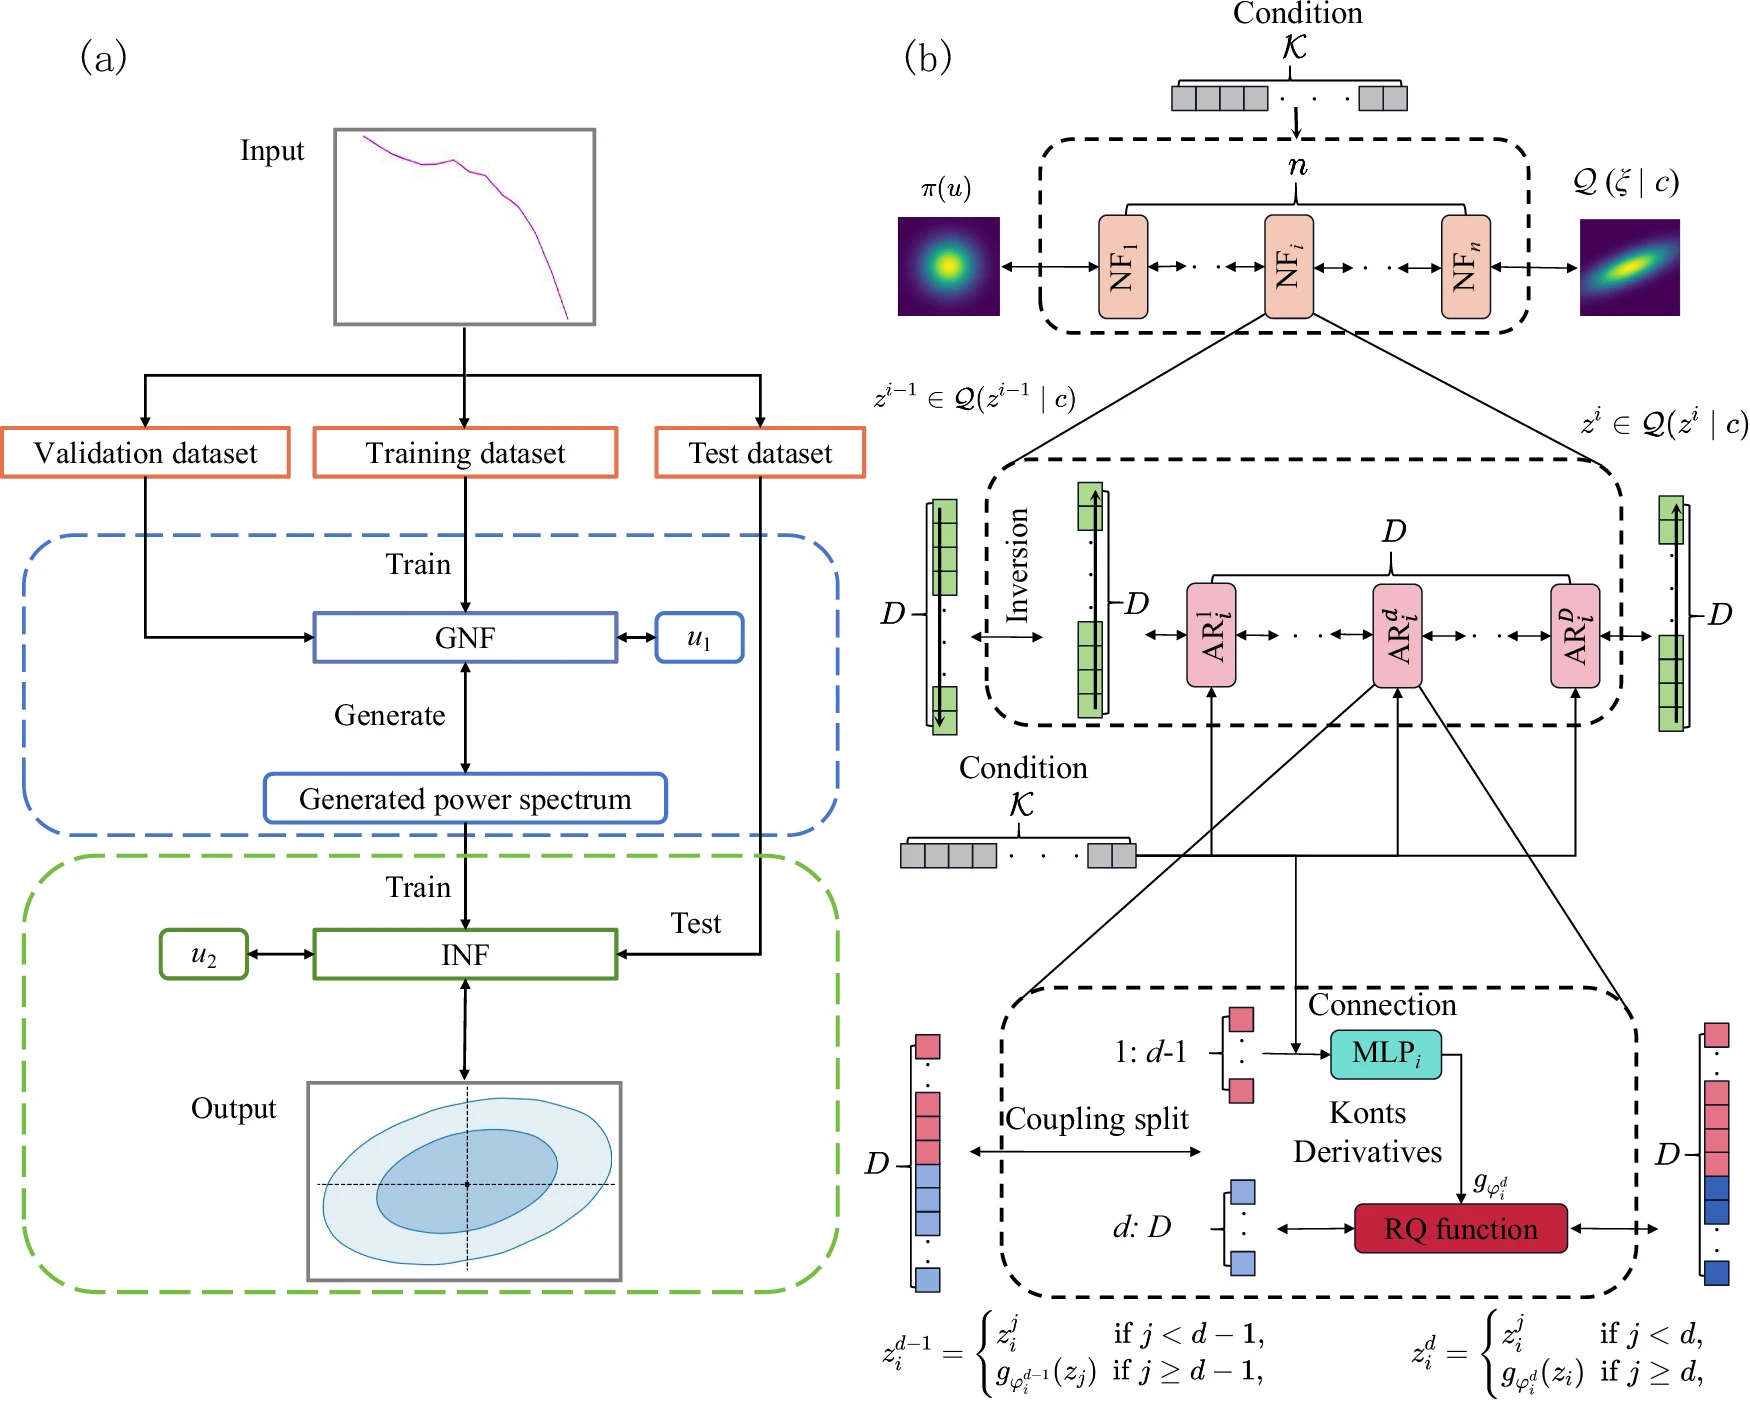
\includegraphics[width=0.96\textwidth]{figures/Sun2025_21cm_fig2.png}
\caption{21cm 森林参数推断中的双流归一化流框架。左图展示从输入功率谱划分训练集、验证集和测试集，并先训练生成归一化流（GNF）扩充模拟样本，再训练推断归一化流（INF）获得参数后验的流程；右图展示条件归一化流及自回归有理二次样条变换模块的结构。该图说明 SBI 方法在“昂贵模拟器+有限训练样本+非高斯后验”问题中的可迁移性。图引自 Sun 等~\cite{sun2025_21cm} 的 Figure 2。}
\label{fig:sbi_transfer_21cm}
\end{figure}

\textbf{CMB功率谱的CVAE异常检测}。跨领域迁移的另一个案例来自宇宙微波背景（CMB）功率谱分析。Sun、Wang 等人~\cite{Sun2025CVAE_CMB}将条件变分自编码器（CVAE）应用于CMB功率谱的宇宙学模型判别与异常检测。CVAE模型能够将CMB功率谱压缩到低维潜在空间，并在其测试设置中实现高保真度重建；对于参数外推情形，其可靠性仍取决于训练覆盖范围和异常判据的校准。这一工作说明，引力波参数估计中发展的CVAE方法论，在结构相近的宇宙学观测问题中也可提供有用工具，并进一步支持“问题结构相似性”是方法迁移成功的重要原因之一。

\textbf{引力波标准汽笛宇宙学综述}。引力波事件作为“标准汽笛”用于宇宙学参数估计，是多信使天文学最重要的科学应用之一。Jin、Wang 等人~\cite{Jin2025GWStandardSirens}系统综述了引力波标准汽笛方法用于哈勃常数等宇宙学参数估计的最新进展，涵盖“亮汽笛”（有电磁对应体）和“暗汽笛”（无电磁对应体）两种方法路线，以及AI方法在提升参数估计精度和处理大样本统计中的关键作用。这一综述为本书第12章关于多信使宇宙学的讨论提供了系统性的文献基础。

\subsection{21cm森林的物理背景与观测挑战}

21cm氢超精细跃迁产生于中性氢原子的电子自旋翻转，静止频率1.42GHz（波长21cm）。高红移（$z=5$--12）的中性氢沿视线方向吸收高红移射电源（如射电类星体）的连续谱辐射，形成“21cm森林”，类似于光学波段的Ly-$\alpha$森林。吸收谱的统计特性（吸收线数密度、等效宽度分布、功率谱）对视线路径上的中性氢密度和气体温度敏感，因此可以约束宇宙再电离历史和暗物质性质。

21cm森林对暗物质性质的约束来自以下物理机制：温暗物质（warm dark matter，WDM）粒子具有非零的自由流长度，会抹平小尺度密度涨落，导致小质量暗物质晕的数量减少。这一效应在21cm森林中表现为：WDM质量越小（自由流长度越大），小尺度吸收特征越少，吸收谱的功率谱在小尺度端越平坦。通过测量21cm森林的功率谱，可以约束WDM粒子质量的下限，目前的约束约为4--5 keV（对应自由流长度约0.1 Mpc）。

21cm森林参数推断面临的主要挑战与引力波参数估计高度相似：模拟代价高昂（单次21cm辐射转移模拟约需1小时，而引力波波形生成约需1毫秒至1秒）；似然函数非高斯（21cm吸收谱的统计分布受非线性结构形成影响，不满足高斯假设）；训练数据稀缺（受计算限制，可用的模拟样本约500条，而引力波参数估计通常使用约 $10^5$--$10^6$ 条训练样本）。

\subsection{SBI迁移的技术实现与结构类比}

Sun等的工作采用双流归一化流架构解决21cm森林参数推断问题。第一个流（生成流）学习从参数空间到观测空间的映射，用于数据增广——从少量真实模拟样本生成大量“虚拟模拟”样本，有效扩充训练集规模。第二个流（推断流）学习从观测空间到参数空间的逆映射，即后验分布 $p(\theta|d)$，用于实际的参数推断。

这一双流架构与引力波参数估计中的SBI方法在结构上高度类比：引力波的观测数据 $d = h(\theta) + n$（信号加噪声），参数 $\theta$ 为源物理参数，模拟器生成 $(\theta, d)$ 对；21cm森林的观测数据为吸收谱，参数为暗物质质量加再电离参数，模拟器生成参数-谱对。两者共享：昂贵模拟、非高斯似然、训练数据稀缺的挑战，以及使用归一化流近似后验分布的技术路线。

在这一迁移过程中，SBI框架的核心思想可以保留，但模拟器（从引力波波形生成器到21cm辐射转移代码）、观测摘要、评估函数（从引力波参数估计精度到21cm功率谱拟合质量）以及校准流程都需要面向新任务重新设计。这种模块化迁移方式，是SBI方法跨领域适用性的一个具体体现。

21cm森林参数推断文章的发表说明，源于引力波数据分析经验的SBI方法已经在独立的物理研究方向上取得同行评议的应用案例，支持了其跨领域应用价值。这提示“引力波AI方法”有机会成为更广泛天文学AI工具箱的一部分，其影响力正在向引力波天文学之外扩展。

SBI方法从引力波到21cm森林的迁移，提示了一个更广泛的方法论原则：在统计推断问题中，“问题结构的相似性”往往比“领域知识的相似性”更有利于方法迁移。引力波参数估计和21cm森林参数推断在物理背景上差异很大——前者涉及强引力场中的致密天体，后者涉及宇宙再电离历史和暗物质性质——但两者共享相近的推断问题结构：给定昂贵的前向模拟器和有限的观测数据，如何高效地推断生成观测数据的物理参数后验分布。这一结构相似性是SBI方法可迁移的重要原因，但并不意味着领域知识可以被忽略；模拟器可信度、观测摘要选择和系统误差建模仍然必须由具体物理问题决定。从这一视角看，SBI方法的跨领域迁移不是简单地“将引力波方法移植到21cm”，而是在两个具体应用场景中实现同一类抽象推断框架。可迁移的是问题求解框架和部分技术组件，而非针对具体问题的完整专用方案。

这一洞察对未来研究有重要启示：引力波数据分析中发展的SBI基础设施（归一化流实现、训练流程、验证框架）可以为其他天文和物理领域提供参考，但通常需要针对领域特定的模拟器、观测数据格式和系统误差重新适配。目前已有初步探索的方向包括：宇宙学大尺度结构的参数推断（用N体模拟替代引力波模拟器）、粒子物理对撞机实验的信号-背景分离（用蒙特卡洛事件生成器替代）、以及地震学中的地壳结构反演（用有限元弹性波模拟替代）。这些方向的进展可能反过来为引力波SBI提供方法论灵感，形成跨领域的方法论共同体。在未来五到十年内，随着跨领域应用积累，“SBI方法学”有望在统计物理、计算天文学和机器学习的交叉处形成更稳定的理论体系和实践规范；引力波数据分析可作为其中较早、较系统的应用场景之一发挥推动作用。

SBI方法跨领域迁移的成功，也给引力波数据分析社区带来了一个重要的学术责任：系统整理和共享方法论工具。当前引力波SBI研究所积累的训练框架、验证工具（PP图生成、覆盖率检验脚本）、和基准数据集，如果能够以开放科学的方式发布，将极大地降低其他领域采用SBI方法的技术门槛，加速跨领域迁移的进程。引力波数据分析社区已经在开放科学方面有良好传统——LIGO-Virgo合作组的引力波事件数据和参数估计结果通过GWOSC（引力波开放科学中心，Gravitational Wave Open Science Center）公开发布，PyCBC、Bilby等分析代码均开源。将这一传统延伸到SBI方法论工具的开放共享，是引力波天文学对整个天文物理AI方法论社区的重要贡献机会。

广义相对论（GR）是迄今最成功的引力理论，但其在强场、高能条件下的完备性仍是开放问题。暗物质、暗能量的存在暗示 GR 可能需要修正，而引力波观测提供了在强场动力学条件下检验 GR 的独特机会。

传统的 beyond-GR 信号搜索面临根本性困难：替代引力理论的数量极多，为每种理论构建专用模板库在计算上不可行。Wang 等人~\cite{wang2025beyondgr} 提出了一种不同的思路：利用在 GR 波形上训练的神经网络的泛化能力，探测偏离 GR 的奇异信号。若网络学习到的是与引力波形态相关的稳健特征，而非训练模板的表面细节，则有可能对部分训练分布之外的信号产生响应。

这一工作的意义超越了具体的方法改进。它展示了 AI 作为弱模型依赖异常筛选工具的潜力：不为每一种替代引力理论预先构建专用模板，而是通过学习已知信号的稳健特征来识别可能偏离训练分布的候选。这一思路与粒子物理中的“模型无关新物理搜索”有相通之处，为 AI 参与基础物理检验提供了新的方法参照。

\subsection{标量-张量引力理论与额外极化模式}

广义相对论预言引力波只有两种极化模式：$+$（plus）极化和 $\times$（cross）极化，对应时空度规的两个独立横向自由度。然而，更广泛的引力理论（如标量-张量理论、$f(R)$引力、Brans-Dicke理论）预言引力波可以有额外的极化模式：标量呼吸模（breathing mode）、标量纵向模（longitudinal mode）、以及矢量模（vector modes）。

在Brans-Dicke理论（最简单的标量-张量理论）中，引力波除了 $h_+$ 和 $h_\times$ 两个张量极化之外，还存在额外的“呼吸模”标量极化。标量极化的振幅与耦合常数 $\omega_{BD}$（Brans-Dicke参数）相关，LIGO对 $\omega_{BD}$ 的约束已达到 $\omega_{BD} > 10^5$，但仍有理论动机探索 $\omega_{BD} \sim 10^3$ 的区间。额外极化的信号特征：频率与张量极化相同（同源辐射），但振幅比 $\epsilon \sim 1/\omega_{BD} \ll 1$，通常远小于张量信号，使得传统模板搜索（仅针对张量极化设计）会系统性地遗漏这类信号。

\subsection{Lorentz破缺与引力子质量的频散效应}

广义相对论预言引力子质量为零，引力波以光速传播，不同频率的引力波以相同速度到达探测器。然而，某些修正引力理论（如双度规引力、Lorentz破缺理论）预言引力子具有非零质量 $m_g$，导致色散关系 $E^2 = p^2c^2 + m_g^2c^4$ 偏离GR的 $E = pc$。

有质量引力子会导致不同频率的引力波以不同速度传播，使得啁啾信号在传播过程中发生频散——低频成分先到达，高频成分后到达，波形的时频关系偏离GR预言。对于传播距离 $D$ 的引力波，频散导致的到达时间差约为：
\begin{equation}
\Delta t \approx \frac{D}{2c} \left(\frac{m_g c^2}{h f}\right)^2,
\end{equation}
其中 $f$ 为引力波频率，$h$ 为普朗克常数。LIGO对引力子质量的约束 $m_g < 1.27 \times 10^{-23}$ eV/$c^2$ 来自对GW150914等事件的相位演化分析。AI检测器通过学习GR波形的典型时频关系，对频散效应引起的偏离天然敏感——任何偏离GR时频关系的信号都会被网络标记为“异常”，无需预先知道偏差的具体形式。

\subsection{Wang等beyond-GR检测的具体结果与方法论意义}

Wang等的beyond-GR检测工作采用了一种“异常检测”（anomaly detection）的思路：在GR双黑洞波形上训练一个自编码器（autoencoder），使其学习GR信号的紧凑表示；对于偏离GR的信号，自编码器的重建误差会显著增大，从而实现检测。

训练集由 $10^5$ 条GR双黑洞波形（注入模拟噪声）组成；测试集包含GR信号和3种beyond-GR信号：额外极化（呼吸模振幅 $\epsilon = 0.01$--$0.1$）、频散效应（引力子质量 $m_g c^2 = 10^{-23}$--$10^{-22}$ eV）、后牛顿偏差（PN系数偏差 $\delta\hat{\phi}_4 = 0.05$--$0.2$）。

在接收者操作特征曲线（ROC）的AUC指标上，对额外极化（$\epsilon=0.1$），检测率约95\%（误报率1\%）；对频散效应（质量 $m_g c^2 = 10^{-22}$ eV），检测率约85\%；对PN偏差（$\delta\hat{\phi}_4 = 0.1$），检测率约90\%。这些结果表明，在该模拟设置中，AI检测器可作为传统模板搜索的补充，用于筛选部分传统模板库难以覆盖的候选信号空间。

这一工作的方法论意义在于：它将引力波数据分析从“验证已知理论”扩展到“探索未知偏差”，为构建较少依赖具体替代理论模板的引力检验工具提供了思路。随着探测器灵敏度的提升和观测事件数量的增加，这类模型无关或弱模型依赖搜索的统计功效有望增强，并可能帮助发现值得进一步精细分析的GR偏差候选或未预期信号。

AI作为弱模型依赖异常筛选工具的价值，在未来的引力波科学中可能随探测灵敏度提升而增长。当探测器能够探测到更远距离（更高红移）的引力波事件时，引力波在传播过程中会对某些偏离GR的效应更加敏感：引力子质量引起的频散效应可随传播距离积累；暗能量或暗物质相关的有效引力修正可能在宇宙学尺度上留下迹象；超出标准模型的新物理（如额外维度）也可能导致传播速度或振幅演化的修正。AI方法若能学习到近距离GR引力波的稳健特征，便可能对某些远距离传播效应引起的异常形态产生响应，从而在缺乏具体理论模板时筛选出值得精细分析的候选事件。这种“AI预筛选+传统精细分析”的两步策略，是未来海量引力波数据中寻找新物理候选的一条可行路径。从实际操作层面看，这一策略的实施需要建立配套的统计框架：AI预筛选输出的“异常候选”需要被赋予统计显著性（如误报率），而后续精细分析的优先级应根据统计显著性和科学价值综合确定。随着AI方法的成熟和验证框架的完善，这一两步策略有望成为未来空间引力波天文台beyond-GR搜索的重要组成部分。

beyond-GR引力波搜索是引力波天文学与基础物理研究的深度交叉点。广义相对论在小尺度（量子引力）和大尺度（暗物质暗能量）两端都面临理论挑战，而引力波探测恰好在两个尺度上都具有灵敏度：双黑洞并合的波形携带了关于紧凑天体附近强引力场（量子引力可能生效的区域）的信息，而引力波在宇宙学距离上的传播则对大尺度引力修正（DE、DM与引力波的耦合）敏感。传统的beyond-GR搜索聚焦于特定理论的具体预言，而人工智能作为弱模型依赖异常筛选工具，可以帮助扩展“偏离GR”候选信号空间，使引力波天文台成为基础物理检验的重要平台之一。随着空间引力波探测器（太极/LISA）的建设，在宇宙学距离（红移$z>5$）上系统性地寻找GR偏差将成为重要的科学目标，而人工智能方法可在候选筛选、异常排序和后续精细分析触发中发挥重要作用。

综合本书各章的工作，可以勾勒出智能化引力波天文学的未来形态。

\textbf{持续智能监测}。未来的引力波天文台将不再依赖人工触发和逐事件分析，而是由 AI 系统持续监测数据流，自动识别信号、估计参数、触发多信使预警。这一系统需要将信号识别（第5章）、参数估计（第6章）、去噪（第7章）、算法自动优化（第8章）有机整合，形成一个自适应的智能管道。

\textbf{自动算法进化}。随着观测数据的积累和噪声特性的变化，数据分析算法需要持续更新。Evo-MCTS 等框架提供了一种机制：以新的观测数据为评估基准，搜索适应当前噪声条件的高性能候选算法，减少完全依赖人工重新设计的负担。

\textbf{跨领域知识融合}。引力波天文学与电磁天文学、中微子天文学、宇宙学的深度融合，将产生新的多信使推断问题。SBI 方法的跨领域迁移能力，使其成为这一融合的天然纽带：同一推断框架可以处理来自不同观测窗口的数据，提取互补的物理信息。

\textbf{人机协作的新模式}。AI 承担算法发现、信号识别、参数估计等计算密集型任务，人类专家专注于科学问题的定义、结果的物理解释、以及新发现的跟进研究。这一分工不是人类被替代，而是人类认知能力的延伸——AI 扩展了人类能够探索的算法空间和信号空间，使科学家能够将精力集中在真正需要物理直觉和创造力的问题上。

\subsection{技术路线图（2025--2035）}

从当前的方法论探索期到未来的工程化成熟期，智能化引力波天文学的技术发展可以划分为三个阶段。

近期（2025--2027年）的重点是完善地面探测器的AI分析管道，建立标准化的SBI推断框架，开展首批太极高保真仿真验证。具体目标包括：在LIGO O4/O5数据或真实噪声注入数据上系统验证SBI方法的统计一致性；建立太极高保真仿真平台（包含TDI实现、时变响应函数、非稳态噪声模型）；完成Evo-MCTS框架在引力波参数估计和去噪任务上的迁移验证。

中期（2027--2030年）的重点是太极/LISA在轨测试数据的AI分析，发展第一代空间引力波在线分析系统，Evo-MCTS框架的系统化和自动化。具体目标包括：实现含100个可分辨银河系双星的中等规模全局拟合（参数维度约 $10^3$）；建立空间引力波数据分析的标准化验证基准（类似地面探测器的MLGWSC-1）；完成三任务（太极+LISA+天琴）联合分析框架的原型验证。

长期（2030--2035年）的重点是面向太极/LISA正式科学运行准备全局拟合管道、多信使联合分析和系统化AI推断。具体目标包括：实现接近任务需求规模的全局拟合原型（可分辨源数约 $10^4$）；建立与SKA等多波段天文台的联合推断平台；完成智能化空间引力波数据处理系统的集成验证，支持从数据采集到候选事件筛选和初步科学产品生成的高度自动化流程。这一三阶段路线图不仅是技术发展的时间表，更是方法论成熟度的评估框架：近期目标对应“单模块验证”阶段，中期目标对应“系统集成原型”阶段，长期目标对应“生产就绪的完整系统”阶段。每个阶段的完成不仅推动了技术进步，也积累了对方法论体系的更深入理解，为下一阶段奠定基础。在这个意义上，本书介绍的方法论创新，都服务于这一更宏大的目标：建造一套能够持续、可靠地探索引力波宇宙的智能化数据分析基础设施。

未来智能化引力波天文台的日常运行将遵循一套人机协作的标准工作流程，在不同时间尺度上分配AI和人类专家的工作。

在秒至分钟的低延迟时间尺度上，AI系统有望承担若干自动化环节：引力波候选体的触发和分类（基于实时信号识别网络）；初步参数估计和天空定位（基于SBI方法或低延迟贝叶斯近似）；多信使预警草案的生成和分发前检查。对于短暂电磁对应体，减少人工和计算延迟十分关键；但预警发布仍需根据数据质量、误报控制和合作组政策设置相应的自动或人工审核机制。

在分钟至小时的时间尺度上，AI辅助人类完成：精确参数估计和不确定度量化（混合AI+贝叶斯，约1--3小时）；信号真实性的交叉验证（多探测器一致性检验、与已知噪声源的对比）；异常事件的专项分析（beyond-GR信号候选、未预期信号形态）。这一层次的人机协作确保了科学结论的可靠性，避免了纯自动化系统可能产生的系统性误差。

在天至周的时间尺度上，人类专家主导：物理解释和科学结论（引力波源的天体物理意义、对基础物理的约束）；算法优化和方法论更新（Evo-MCTS周期性自动优化，人类专家季度审查）；科学论文的撰写和同行评审。这一层次的人类主导确保了科学发现的深度和可信度，是AI无法替代的核心价值所在。

\subsection{下一代技术的潜在影响}

除本书系统介绍的方法之外，若干新兴 AI 技术在引力波数据分析中具有重要的潜在价值，值得在此展望。

\textbf{扩散模型（Diffusion Models）}。近年来在图像生成领域取得突破性进展的扩散模型，其核心思想是学习从噪声分布到目标分布的去噪路径，天然适合引力波去噪任务。与 WaveFormer 等判别式去噪方法不同，扩散模型是生成式的：它能够为同一含噪输入生成多个去噪样本，从而提供去噪结果的不确定度估计。这一特性对于评估去噪后参数估计的可靠性具有重要意义。扩散模型用于 SBI 也正在成为活跃的研究方向，其在 EMRI 等多模态后验分布的建模上可能优于标准归一化流。

\textbf{基础模型（Foundation Models）}。大语言模型在代码生成和候选算法搜索方面的能力，已通过 Evo-MCTS 框架在引力波算法发现中得到初步验证。更进一步，针对物理科学数据训练的“物理基础模型”（physics foundation model）——在大量物理模拟数据上预训练的通用模型——有望提供一种更统一的数据分析范式：从原始或低级预处理后的探测器数据中学习通用表示，再服务于检测、参数估计、去噪和异常识别等下游任务。其科学使用仍需要严格的物理约束、校准验证和可解释性评估。

\textbf{多模态天文学中的 AI 协同}。随着电磁天文台（SKA、ELT、CSST）和中微子探测器（IceCube）灵敏度的持续提升，多信使天文学将从“偶发的联合观测”演变为“系统性的跨波段推断”~\cite{Abbott2017GW170817}。引力波数据分析中发展的 SBI 框架，与电磁和中微子观测的联合推断，是这一方向的自然延伸：同一贝叶斯框架可以同时处理来自不同探测器的数据，提取关于引力波源的互补物理信息——例如，同时利用引力波信号确定双中子星并合的质量参数，利用千新星光变曲线约束核物质状态方程，利用短伽马射线暴喷流结构推断黑洞自旋。

\textbf{量子计算的远期展望}。量子计算在某些特定类型的组合优化、采样和线性代数问题上具有理论加速可能。对于引力波数据分析中的某些高维积分或模板放置问题，量子蒙特卡洛、量子退火或量子近似优化算法可以作为远期探索方向。尽管这一方向目前仍处于基础研究阶段，距离实际应用尚有较大距离，且尚无引力波数据分析中的量子优势实验证据，但量子计算与 AI 方法的结合（量子机器学习）仍是远期技术路线图中值得关注的方向。

引力波天文学的未来，是人类智慧与人工智能深度协作的未来。本书所呈现的方法论体系，正是这一协作的早期实践与系统总结。

在科学目标层面，未来十年内最令人期待的进展包括以下几个方向。第一，引力波背景的多频段观测：脉冲星计时阵列（PTA）在纳赫兹频段已发现随机引力波背景的候选信号，太极/LISA在毫赫兹频段可能探测到宇宙相变或弦网络背景，两者的联合约束将为早期宇宙物理提供新的观测窗口。第二，极端质量比旋近的第一批系统性探测：EMRI是空间引力波探测器的“旗舰”科学目标，每个EMRI事件携带的强引力场信息相当于在黑洞附近进行数十万圈的精密轨道力学测量，AI方法（特别是CNF参数估计）是使这一科学目标从“理论上可能”变为“实际可分析”的关键使能技术。第三，多信使宇宙学：利用引力波事件作为“标准汽笛”对宇宙学距离进行测量，既包括有电磁对应体的“亮汽笛”，也包括依赖星系目录和统计关联的“暗汽笛”。当事件数量和星系红移信息足够丰富时，哈勃常数测量精度有望逐步接近百分之几乃至百分之一量级，为检验哈勃张力提供独立信息。

从方法论演进的角度看，AI在引力波天文学中的应用正在从“方法移植”（将通用AI方法移植到引力波场景）向“方法创生”（由引力波特定问题催生新的AI方法论范式）演进。MF-CNN的感知层设计、SBI与贝叶斯的精确协同、Evo-MCTS的可解释算法自动发现，都是引力波物理的独特挑战催生的方法论创新，这些创新反过来又为更广泛的科学AI方法论贡献了新的视角和工具。这种从“领域应用”到“方法创生”的转变，标志着引力波数据分析已经从AI技术的“消费者”成长为AI方法论的“生产者”。

\begin{table}[htbp]
\centering
\caption{引力波天文学AI方法论里程碑总结}
\label{tab:ai_milestones}
\small
\begin{tabular}{llll}
\hline
\textbf{方法} & \textbf{代表工作} & \textbf{关键成果} & \textbf{科学意义} \\
\hline
MF-CNN & Wang等 (2020) & 识别O1/O2多数确认事件 & 物理先验嵌入范式 \\
集成学习 & Ma等 (2022) & 跨轮次低误报泛化 & 鲁棒性验证 \\
SBI归一化流 & Wang等 (2022) & 高维参数估计加速 & 推断范式转变 \\
WaveFormer & Wang等 (2024) & 全局时频特征捕获 & Transformer在GW去噪中的应用 \\
CNF-EMRI & Liang等 (2024) & 17维参数估计探索 & 空间GW分析可行化 \\
混合推断 & Sun等 (2025) & 采样时间压缩至14\% & 精确协同范式 \\
Evo-MCTS & Wang等 (2025) & 超越既有ML基线20.2\% & AI驱动算法发现 \\
\hline
\end{tabular}
\end{table}

\section{下一代探测器与人工智能方法的协同演化}

\begin{figure}[htbp]
\centering
\resizebox{0.98\textwidth}{!}{%
\begin{tikzpicture}[
  font=\small,
  milestone/.style={draw, rounded corners=3pt, text width=25mm, minimum height=10mm,
                    text centered, align=center, fill=blue!8, draw=blue!45,
                    font=\scriptsize, inner sep=2.5pt},
  future/.style={draw, rounded corners=3pt, text width=25mm, minimum height=10mm,
                 text centered, align=center, fill=orange!10, draw=orange!60,
                 dashed, font=\scriptsize, inner sep=2.5pt},
  arr/.style={-Stealth, thick, gray!60},
]
% 时间轴
\draw[-Stealth, very thick, gray!55] (0,0) -- (15.2,0)
  node[right,font=\scriptsize,gray!70]{时间};
\foreach \x/\yr in {0.8/2020, 3.2/2022, 6.4/2024, 9.8/2025, 12.6/2030, 14.4/2035} {
  \draw[gray!45, thin] (\x,-0.12) -- (\x,0.12);
  \node[font=\scriptsize, gray!75] at (\x,-0.35) {\yr};
}

% 里程碑
\node[milestone] (mfcnn) at (0.8,1.35) {MF-CNN\\物理先验嵌入};
\node[milestone] (normflow) at (3.2,-1.35) {归一化流\\SBI参数估计};
\node[milestone] (waveformer) at (5.6,1.35) {WaveFormer\\Transformer去噪};
\node[milestone] (cnfemri) at (7.5,-1.35) {CNF-EMRI\\17维参数估计};
\node[milestone] (evomcts) at (10.0,1.35) {Evo-MCTS\\自动算法发现};

% 未来里程碑
\node[future] (globalfit) at (12.5,-1.35) {全局拟合原型\\$10^4$量级联合推断};
\node[future] (realtime) at (14.2,1.35) {实时智能管道\\低延迟自动化};

% 连接线
\draw[arr] (0.8,0.12) -- (mfcnn.south);
\draw[arr] (3.2,-0.12) -- (normflow.north);
\draw[arr] (5.6,0.12) -- (waveformer.south);
\draw[arr] (7.5,-0.12) -- (cnfemri.north);
\draw[arr] (10.0,0.12) -- (evomcts.south);
\draw[arr, dashed, orange!70] (12.5,-0.12) -- (globalfit.north);
\draw[arr, dashed, orange!70] (14.2,0.12) -- (realtime.south);
\end{tikzpicture}}
\caption{引力波AI方法论里程碑时间线。蓝色实线框为本书讨论的已发表或已完成研究工作，橙色虚线框为面向下一代探测器和空间引力波任务的阶段性研究目标。从MF-CNN到Evo-MCTS，相关工作展示了从“物理先验嵌入”到“自动算法发现”的方法论拓展；未来节点为路线图式概括，并非任务正式时间表。代表性工作参见文献~\cite{wang2020deeplearning,wang2022normflow,wang2024waveformer,liang2024cnfemri,sun2025cvae,wang2025evomcts,wang2024challenges,du2026taiji}。}
\label{fig:ai_timeline}
\end{figure}

下一代地面引力波探测器——爱因斯坦望远镜（ET）~\cite{Punturo2010ET} 和宇宙探索者（CE）~\cite{Evans2021CE}——计划在2030年代推进建设，其灵敏度目标比 Advanced LIGO 提升约一个量级，预期事件率可能达到每年 $10^5$ 量级或更高。这一量级的事件率将使当前的逐事件人工分析模式难以维系，人工智能方法有望从“辅助工具”发展为数据分析基础设施中的核心组成部分。

\textbf{ET/CE 对数据分析的新要求}。ET 采用三角形地下配置，三条臂长10公里的干涉仪，低频截止目标约2--3 Hz，使其能够探测更长的双中子星旋进信号和更高红移的双黑洞。CE 采用L型配置，臂长40公里，在宽频段提供高灵敏度，与ET形成互补。两者联合运行时，双中子星和双黑洞事件数将大幅增加，其中一部分可望具有电磁对应体，多信使天文学将从“偶发事件”演变为“统计样本”。

对数据分析的新要求体现在三个方面：（1）\textbf{实时性}——多信使预警需要在并合前或并合后极短时间内完成参数估计，SBI方法的快速推断提供了一条具有吸引力的技术路线；（2）\textbf{可扩展性}——每年 $10^5$ 量级事件的参数估计需要高度自动化的流水线，人工干预应主要集中于科学价值最高或最异常的事件；（3）\textbf{精度}——更高灵敏度意味着更高信噪比，参数估计精度要求相应提升，SBI方法的精度验证（PP图检验）将成为科学可信度的重要保障。

\textbf{AI方法的协同演进路径}。面向ET/CE时代，AI方法需要在以下方向协同演进：归一化流架构需要扩展到更高维度（包含潮汐形变参数的BNS系统约17维）；训练数据需要覆盖更宽的参数范围（高红移、高质量比、高自旋）；实时推断系统需要与多信使预警基础设施深度集成；可靠性工程需要建立与经典方法等同级别的验证框架。这些演进方向，正是本书各章方法论工作的自然延伸，也是未来引力波AI研究最重要的工程目标。

\begin{table}[htbp]
\centering
\caption{下一代引力波探测器与AI方法需求对比}
\label{tab:next_gen_detectors}
\small
\begin{tabular}{lcccc}
\hline
\textbf{探测器} & \textbf{臂长} & \textbf{低频截止} & \textbf{年事件率} & \textbf{AI关键需求} \\
\hline
Advanced LIGO O4 & 4 km & $\sim$10 Hz & 百量级公开候选 & 辅助加速 \\
爱因斯坦望远镜（ET） & 10 km（地下） & $\sim$2--3 Hz & $\sim 10^5$量级 & 高度自动化 \\
宇宙探索者（CE） & 40 km & $\sim$5 Hz & $\sim 10^5$量级 & 高度自动化 \\
太极/LISA & 百万 km（空间） & 毫赫兹窗口 & 依源类而定 & 全局拟合 \\
\hline
\end{tabular}
\end{table}

\section{量子传感与引力波探测的未来}

引力波探测的灵敏度提升，在经典物理框架内已接近基本极限。地面引力波探测器的噪声预算由量子噪声（散粒噪声和辐射压力噪声）、热噪声和地震噪声共同决定，其中量子噪声在宽频段内占主导地位。突破经典极限、进入量子增强探测的新时代，是下一代引力波探测器的核心技术挑战，也是量子光学、原子物理与引力波天文学深度交叉的前沿领域。

\subsection{量子压缩光的现状与前景}

量子压缩光技术是目前最成熟的量子增强引力波探测方案，已在Advanced LIGO的O3观测运行中实现了工程化应用。在标准量子极限（SQL）框架下，迈克尔逊干涉仪的量子噪声由海森堡不确定性原理约束：
\begin{equation}
\Delta x \cdot \Delta p \geq \frac{\hbar}{2},
\end{equation}
其中$\Delta x$为位置（相位）不确定度，$\Delta p$为动量（振幅）不确定度。标准相干光的量子噪声在相位和振幅两个正交分量上均等分布；压缩光通过非线性光学过程（参量下转换）将量子噪声从相位分量“压缩”到振幅分量，从而在牺牲振幅精度的代价下提升相位（即引力波信号）的测量精度。

Advanced LIGO O3运行期间，注入15 dB的压缩光（对应量子噪声降低约$10^{15/10}\approx32$倍的功率，即约5.6倍的振幅）使探测器在高频段（$>$50 Hz）的灵敏度提升约3倍信噪比~\cite{Tse2019squeezing}。这一成果标志着量子增强引力波探测从实验室演示走向实际科学运行的历史性跨越。然而，15 dB压缩在实践中受到光学损耗（镜面散射、吸收）和相位噪声的严格限制，进一步提升压缩度面临工程上的系统性挑战。

量子反作用规避（Quantum Non-Demolition，QND）技术代表了超越标准量子极限的更深层次方案。在标准迈克尔逊干涉仪中，测量光子对镜面施加辐射压力，产生量子反作用噪声；在高功率运行时，辐射压力噪声与散粒噪声的乘积恰好等于标准量子极限。QND技术通过设计特殊的光学配置，使辐射压力噪声与散粒噪声之间产生量子相关（quantum correlation），从而在原理上突破标准量子极限。变速光（speed meter）配置是QND技术的一种具体实现：通过在干涉仪中引入额外的“速度测量”光路，使探测器对镜面速度（而非位置）敏感，从而规避辐射压力反作用的影响。理论分析表明，理想的QND探测器可以将灵敏度提升至海森堡极限：
\begin{equation}
\Delta x_{\rm Heisenberg} = \frac{\hbar}{2\Delta p} \propto \frac{1}{\sqrt{N_{\rm photon}}},
\end{equation}
其中$N_{\rm photon}$为探测光子数，对应灵敏度随光功率的平方根提升，而非标准量子极限下的线性关系。爱因斯坦望远镜（ET）和宇宙探索者（CE）的设计方案均将QND技术列为核心技术路线，预期在2030年代实现工程化验证。

\subsection{原子干涉引力波探测器}

原子干涉仪利用超冷原子的物质波干涉效应测量引力波引起的时空应变，代表了不同于激光干涉仪的技术路线。在原子干涉仪中，激光脉冲将原子波包分裂、偏转和重合，形成类似于光学迈克尔逊干涉仪的干涉结构；引力波引起的时空应变改变了两条原子路径的相对相位，从而在干涉条纹中留下可测量的信号。原子干涉仪的潜在优势在于：原子的内部量子态（超精细能级）可提供稳定的相位参考，并在特定设计下改善低频加速度噪声（地震噪声、重力梯度噪声）对测量的影响。

当前国际上主要的原子干涉引力波探测器项目包括：英国的AION（Atom Interferometer Observatory and Network）~\cite{Badurina2020AION}，计划建设10米、100米和1公里三个尺度的原子干涉仪，逐步验证从实验室到引力波探测的技术路线；美国的MAGIS（Mid-band Atomic Gravitational wave Interferometric Sensor）~\cite{Graham2017MAGIS}，利用斯坦福大学的100米垂直塔开展原型验证，目标是在0.1--10 Hz的中频段实现引力波探测；中国的ZAIGA（Zhaoshan Long-baseline Atom Interferometer Gravitation Antenna）~\cite{Zhan2020ZAIGA}，依托武汉赵山地下实验室建设，利用地下环境的低地震噪声优势，计划实现基线长度达数百米的原子干涉仪网络。

原子干涉引力波探测器的独特科学价值在于其对中频段（0.1--10 Hz）的灵敏度。这一频段恰好处于地面激光干涉仪（灵敏频段$>$10 Hz）和主要面向毫赫兹频段的空间激光干涉仪之间，是当前引力波探测网络的重要盲区。中频段的主要科学目标包括：中等质量黑洞（IMBH，$10^2$--$10^5\,M_\odot$）的并合信号——这类天体的存在是连接恒星质量黑洞（$\sim$10$M_\odot$）和超大质量黑洞（$>10^6\,M_\odot$）的关键环节，但迄今尚无确凿的引力波探测证据；双中子星并合的早期旋近阶段——在地面探测器灵敏频段之前数小时至数天，原子干涉仪可以提前预警，为多信使观测提供充裕的准备时间；以及宇宙学引力波背景的中频段成分，对早期宇宙相变和宇宙弦网络的约束能力远超现有探测器。

\subsection{量子网络与引力波天文学}

量子网络技术与引力波天文学的交叉，开辟了超越单台探测器灵敏度极限的新可能性。量子纠缠辅助的探测器网络是一个远期设想：通过在地理上分离的探测器之间分发量子关联资源，理论上可改善联合测量的量子噪声表现。由于长距离纠缠分发、光学损耗、相位稳定和探测器耦合都极具挑战，这一方向目前主要停留在理论和概念验证阶段。

量子通信技术在引力波预警系统中的应用，目前更接近信息安全层面的远期设想。当前引力波预警系统依赖经典通信网络传输候选事件和天空定位信息，其主要瓶颈通常来自数据处理、候选审核和望远镜调度，而非加密方式本身。量子密钥分发（QKD）可为高安全需求的科学通信提供一种可能方案，但它不是提升多信使预警时效性的核心技术路径。

量子计算加速引力波数据分析，是量子技术与引力波天文学交叉中具有长期潜力、但也高度不确定的方向。量子机器学习算法在特定输入模型和数据访问假设下可能提供复杂度优势，量子蒙特卡洛方法也可能加速某些高维积分估计。然而，这些理论优势往往依赖强假设（如高效量子数据加载、低噪声深电路或特定问题结构），目前尚不能直接转化为引力波参数估计或搜索流水线中的实际加速。

\subsection{AI与量子技术的协同}

量子机器学习用于引力波参数估计的理论可行性，是近年来量子计算与引力波天文学交叉研究的核心问题。量子神经网络（QNN）通过参数化量子电路（PQC）实现类似经典神经网络的函数逼近能力，其表达能力在理论上由量子电路的纠缠结构决定。对于引力波参数估计问题，QNN的潜在优势在于：量子态的希尔伯特空间维度随量子比特数指数增长，使得QNN在原理上可以用较少的参数表达经典神经网络需要大量参数才能表达的复杂函数；量子纠缠可以自然地编码引力波参数之间的相关性（如质量比与自旋之间的简并），从而提升参数估计的效率。

然而，量子优势的实际实现面临近期量子计算机的严峻限制。当前NISQ设备虽然已具备数百到上千量级物理量子比特的实验平台，但量子退相干、门错误率和读出误差限制了可执行电路深度；容错逻辑量子比特的规模仍远不足以处理引力波参数估计这类复杂科学计算问题。更根本的挑战在于：许多量子机器学习的理论加速优势依赖于高效量子数据加载或QRAM，而这些条件在实际硬件上仍是开放工程难题。

从更现实的近期视角来看，量子-经典混合算法（variational quantum algorithms，VQA）代表了在NISQ时代最有可能实现实际应用的量子计算路线。VQA将量子电路用于计算经典计算机难以高效处理的特定子任务（如量子态制备、量子核函数计算），而将优化和后处理留给经典计算机，形成量子-经典协同的计算架构。在引力波数据分析中，VQA的潜在应用包括：利用量子核方法加速引力波信号的特征提取、利用量子采样加速贝叶斯后验的低维投影计算，以及利用量子优化算法改进引力波模板库的覆盖策略。

AI与量子技术的协同，在更深层次上体现为两种技术路线的互补性：AI方法（特别是深度学习和SBI）擅长处理高维、非线性的数据分析问题，但受限于经典计算资源；量子计算在特定问题上具有理论加速潜力，但受限于当前量子硬件的噪声和规模。两者的协同可以从识别适合量子加速的低维子任务开始，例如小规模组合优化、低维积分或核函数估计。这一融合的实现，需要引力波物理学家、量子计算研究者和AI研究者的深度跨学科合作，也需要量子硬件技术的持续进步。就当前技术状态而言，它更应被视为长期探索方向，而非太极/LISA早期数据处理的近期方案。

\section{引力波天文学与多信使科学的深度融合}

多信使天文学（multi-messenger astronomy）是引力波天文学最重要的科学应用场景之一，也是AI方法发挥关键作用的核心领域。GW170817双中子星并合事件的成功多信使观测，已经展示了引力波与电磁波联合分析的巨大科学价值；而未来随着探测器灵敏度的提升和AI方法的成熟，多信使天文学将从“偶发事件”演变为“系统性科学”。

\textbf{多信使预警的时效性要求}。双中子星并合事件在并合前数分钟至数小时内，旋进阶段的引力波信号已经进入LIGO/Virgo的灵敏频段。对于典型的BNS系统（总质量约$2.8\,M_\odot$），信号在并合前约15分钟进入10 Hz频段，在并合前约1分钟进入100 Hz频段。如果能在并合前数分钟内完成参数估计并发出预警，电磁望远镜可以提前指向目标天区，捕捉并合瞬间的伽马射线暴（GRB）和千新星（kilonova）的早期辐射——这些早期辐射携带了关于中子星物质状态方程和重元素核合成的关键信息，是事后观测无法获取的。

SBI方法的快速推断速度，使并合前实时参数估计成为有吸引力的技术目标。一个可设想的流程是：在线匹配滤波或CNN检测器识别BNS候选体，SBI归一化流给出快速近似参数后验，BAYESTAR等低延迟天空定位工具给出初步定位，然后向全球电磁望远镜网络发送预警。实际总延迟取决于信号进入频段的时间、触发阈值、数据质量检查、人工或自动审核策略以及望远镜调度系统，因此不宜用单一固定时间概括；但AI快速推断有望压缩其中的参数估计环节。

\textbf{引力波标准汽笛与哈勃常数测量}。引力波事件提供了一种独立于传统距离阶梯的宇宙学距离测量方法——“引力波标准汽笛”（gravitational wave standard siren）。双中子星并合事件的引力波波形直接编码了光度距离信息（通过波形振幅），无需依赖传统距离阶梯校准。结合电磁对应体确定的宿主星系红移，可以独立测量哈勃常数$H_0$。GW170817给出$H_0$的十余个百分点精度约束；随着BNS事件数量、星系红移目录和暗汽笛统计方法的发展，标准汽笛有望逐步提高$H_0$测量精度，并为检验CMB测量与传统距离阶梯测量之间的“哈勃张力”提供独立证据；可达到的具体精度仍取决于事件样本、宿主星系关联、选择效应和系统误差控制。

AI方法在标准汽笛分析中的关键作用体现在两个方面：其一，SBI方法对BNS事件的快速参数估计（特别是距离和倾角的联合后验），有助于积累大样本统计；其二，机器学习方法对宿主星系候选筛选、星系目录匹配和红移信息整合具有潜在价值，可在没有明确电磁对应体的情况下通过统计方法（“暗汽笛”方法）利用更多引力波事件约束$H_0$。

\textbf{中子星状态方程的多信使约束}。双中子星并合事件对中子星物质状态方程（EOS）的约束，是多信使天文学最重要的核物理科学目标之一。引力波波形在并合前最后几个轨道周期内对潮汐形变率$\Lambda$敏感，$\Lambda$反映了中子星的内部结构（半径和可压缩性）。GW170817对$\Lambda$的测量已将典型中子星半径约束到十余公里量级，并排除了一部分极端状态方程。未来ET/CE时代，多事件联合分析有望显著改善半径和EOS参数约束，但具体精度取决于事件数、信噪比分布、波形系统误差和电磁对应体信息。

AI方法在EOS约束中的作用包括：SBI方法对包含潮汐形变参数的BNS波形（约17维参数空间）的快速参数估计；机器学习方法对千新星光变曲线的自动分析（约束重元素产率和喷射物质量）；以及贝叶斯层级分析框架对大量BNS事件的联合EOS约束。这些方法的协同，将使多信使BNS分析从“单事件精细研究”升级为“大样本统计科学”，是引力波天文学与核物理学深度融合的技术基础。

\section{本章小结}

本章从四个维度展望了智能化引力波天文学的发展趋势：LLM驱动的自动算法发现、SBI方法的跨领域迁移、弱模型依赖信号探测，以及智能化天文学的未来形态。人工智能在引力波天文学中的角色演变不是线性改进，而是结构性扩展——从“计算工具”到“方法协作者”，从“单领域专用”到“跨领域迁移”，从“事后分析”到“低延迟预警”。这三重转变，共同定义了智能化引力波天文学的主要特征，也指向了未来引力波AI研究的重要发展方向。

引力波天文学在AI方法论发展中的独特贡献，部分来自其数据特性的独特组合：信号形态有精确的物理理论支撑（广义相对论+数值相对论），噪声特性有可量化的统计模型，评估标准客观明确且国际公认（MLGWSC-1等挑战赛），物理可解释性要求极为严格（因为科学结论需要同行信任）。这一独特组合使引力波数据分析成为AI方法论探索的理想试验场——既有足够的复杂度来挑战AI方法的能力边界，又有足够的物理约束来验证AI方法的可信度。未来，随着引力波AI方法论的成熟，这一试验场将向更广泛的天文学和物理学领域辐射，推动科学AI方法论从引力波天文学走向更宏大的科学舞台。

引力波天文学与人工智能的深度融合，在更广泛的意义上代表了当代科学探索的一种新范式：面对数据规模和复杂度持续超越人类直接分析能力的科学问题，人工智能不是替代科学家，而是以“认知放大器”的形式扩展科学家的探索能力。引力波数据分析中的AI应用已经展示了这种放大效应的多个维度：计算速度的放大（SBI将若干参数估计任务压缩多个量级）、探索广度的放大（Evo-MCTS在人类难以穷举的算法空间中发现新解）、以及感知深度的放大（可解释性分析揭示网络学到的物理相关特征）。这三个维度的放大，共同构成了智能化引力波天文学的重要方法论基础。

回顾本书记录的方法论演进，从2020年的MF-CNN到2025年前后的Evo-MCTS，引力波AI方法论经历了从“单点性能优化”到“方法论体系建设”的明显推进。这一推进不是由单个结果驱动的，而是多个方向研究的协同积累：可解释性研究建立了物理-AI一致性的验证框架，SBI方法缓解了计算瓶颈，Evo-MCTS展示了自动算法发现的新可能。未来的引力波AI研究，需要在这一基础上继续深化：更精密的可解释性分析（从“定性验证”到“定量约束”）、更可靠的SBI精度保证（从“经验验证”到“理论保证”）、更广泛的自动算法发现应用（从“单任务原型”到“多任务系统”）。这三个方向的协同深化，将支撑太极/LISA时代的海量科学数据处理。

引力波AI方法论的成熟，将从三个层面改变引力波天文学的科学实践模式。在个体研究者层面，AI工具的普及有望降低引力波数据分析的技术门槛，使更广泛的科学社区能够参与这一领域；在合作组层面，AI自动化流水线将压缩从数据采集到初步科学结论的时间周期，加快候选事件筛查和后续观测触发；在学科层面，AI方法的跨领域迁移能力（引力波→21cm森林→更多宇宙学观测）将推动引力波数据分析方法论成为更广泛的天文学AI基础设施的一部分。

第11章的核心论点是：人工智能在引力波天文学中的角色演变不是线性改进，而是结构性扩展。从“计算工具”到“方法协作者”的转变，体现在Evo-MCTS等方法能够搜索候选算法、beyond-GR探测能够作为弱模型依赖检验的辅助工具、SBI方法能够迁移到21cm森林等宇宙学观测问题。LLM驱动的自动算法发现揭示了两条原则：可迁移的是搜索机制而非固定管道，领域知识集成是决定成败的关键因素。智能化引力波天文学的未来形态包括持续智能监测、自动算法优化、跨领域知识融合和人机协作新模式；其核心是扩展人类能够探索的算法空间和信号空间，而非替代人类的物理直觉和创造力。

\chapter{结语：面向可信智能引力波天文学}

\section{本书主要贡献总结}

本书以“人工智能与统计推断的交叉融合”为主线，系统梳理了引力波天文学数据分析方法论的前沿进展。从第一部的理论基础出发，经由第二部对经典方法局限性的深入分析，到第三、四部对 AI 新方法及其与物理融合的系统介绍，最终以第五部对未来挑战与发展趋势的展望收尾——全书构成一个逻辑完整、层次递进的方法论体系。

本书写作的学术背景，是引力波天文学从发现阶段走向大样本和空间探测阶段的关键时期：从2015年GW150914的首次直接探测，到即将到来的太极/LISA空间引力波探测器时代，数据分析面临的计算挑战从“困难但可解决”演变为“直接传统流程难以承担”。正是这种现实需求，驱动了本书所介绍的每一个方法论创新——每一项创新都不是为了创新而创新，而是为了解决引力波天文学前进道路上的具体障碍。这种“问题驱动的方法论创新”精神，贯穿了本书的始终，也是评价这些方法论价值的正确标准。

引力波天文学的成功，既是探测器技术的胜利（将应变灵敏度提升至$10^{-23}$量级），也是数据分析方法的胜利（从海量噪声数据中提取微弱的时空信号）。本书所记录的人工智能方法论创新，是这一数据分析方法演进中的重要组成部分。它们的价值不在于制造技术噱头，而在于把新的计算工具放回引力波天文学的严格物理和统计约束之中，检验其是否真正能够服务于可靠的科学发现。

在方法论层面，本书的核心贡献可以归纳为三条主线。

\textbf{第一条主线：从黑箱到可解释}。早期深度学习方法在引力波数据分析中以高效见长，但决策逻辑对物理学家不透明。本书系统介绍了可解释性的多种实现路径：感知层设计将物理先验以归纳偏置的形式嵌入网络结构~\cite{wang2020deeplearning}（第5章）；随机森林特征分析揭示了 CNN 关注的物理特征~\cite{tian2025cnn}（第5、9章）；Evo-MCTS 框架通过树结构进化搜索，直接发现由可检视模块组成的算法~\cite{wang2025evomcts}（第8章）。这一从“黑箱”到“可解释”的演进，是引力波 AI 方法走向实际科学应用的必经之路。

\textbf{第二条主线：从近似替代到精确协同}。SBI 方法（第6章）和混合推断策略（第6、9章）展示了 AI 与经典贝叶斯方法的一种有代表性的合作模式：神经网络不是替代贝叶斯推断，而是作为快速先验约束工具，在特定实验设置中将精确贝叶斯采样的计算代价压缩至 14\%~\cite{sun2025cvae}。这一“精确协同”范式，相比单纯的“近似替代”更容易满足科学可信度和可校准性的要求。

\textbf{第三条主线：从单一方法到自动发现}。Evo-MCTS（第8章）代表了一种新的方法搜索范式：在由人类专家定义的搜索空间、评估指标和物理约束下，由 LLM 引导的进化搜索提出候选算法~\cite{wang2025evomcts}。在 MLGWSC-1 基准~\cite{schafer2023mlgwsc1}上 20.2\% 的性能提升，说明“AI 辅助算法发现”可以在受控基准中形成可检验的研究路径。

本书系统介绍的方法论体系在科学可信度方面也进行了建设，这是AI方法在严肃科学中应用的重要前提，却往往在方法论论述中被忽视。可信度建设体现在三个层面：统计验证层面，PP图、覆盖率检验、Gelman-Rubin统计量等工具被用于检验AI方法的统计一致性；物理验证层面，遮罩实验、随机森林特征分析、beyond-GR泛化测试等工具被用于考察AI方法的物理一致性；工程验证层面，MLGWSC-1等标准化挑战赛提供了与独立基线的客观比较，增强了性能声明的可重复性。这三个层面的系统验证，构成了引力波AI方法科学可信度的闭环，也是本书对引力波AI方法论的重要贡献之一。科学可信度的建设不应被视为方法开发完成后的附加环节，而应贯穿整个方法论体系的设计之中：从最初的网络架构选择（物理先验的嵌入方式决定了可解释性的深度），到训练策略的制定（训练集的代表性决定了统计一致性的范围），到验证实验的设计（挑战赛的规范性决定了性能声明的可信度）。这种“可信度优先”的方法论设计理念，是引力波数据分析对科学AI方法论的重要贡献之一。

\subsection{MF-CNN的方法论意义}

MF-CNN的核心贡献不仅是“更快的引力波检测器”，而是提供了一个示范性的方法论框架——如何将物理先验以“软约束”（归纳偏置）而非“硬约束”的形式嵌入神经网络~\cite{wang2020deeplearning}。传统的物理约束通常以硬约束的形式出现：要求网络输出满足特定的物理方程，或者在损失函数中加入物理约束项。这种硬约束方式虽然保证了物理一致性，但限制了网络的表达能力，可能导致在复杂噪声条件下的性能下降。

MF-CNN的感知层设计采用了不同的思路：将匹配滤波的三步操作（白化、模板卷积、归一化）实现为可学习的卷积单元，使网络在初始化时具有匹配滤波的行为，但在训练过程中可以根据数据自适应调整。这种“软约束”方式既保留了物理先验的指导作用，又允许网络学习超越匹配滤波的特征表示，在真实噪声条件下表现出更强的鲁棒性。

这一框架的可迁移性在于：许多具有已知物理结构的信号处理问题都可以借鉴类似的“感知层”设计思路。在引力波去噪（WaveFormer）、EMRI检测（两层CNN）、以及空间引力波全源检测（多阶段自注意力网络）中，都可以看到类似的物理先验嵌入策略。对可解释性的贡献同样重要：通过设计物理上有意义的网络结构，MF-CNN的决策逻辑对物理学家更透明、更容易验证，为AI方法在科学应用中的可信度建设提供了基础。

\subsection{SBI方法体系的贡献层次}

SBI方法体系的贡献可以从技术、方法论、科学和跨领域四个层次来理解，每个层次都有其独特的价值。

在技术层次，NPE/CNF/流匹配构成的方法工具箱~\cite{wang2022normflow,du2024normflow,liang2024cnfmbhb,liang2024cnfemri}，将引力波参数估计从“数小时到数年”压缩到“秒级”。这一计算效率的量级提升，使得原本在计算上不可行的分析任务（如EMRI 17维参数估计、空间引力波全局拟合的子问题）变得实际可行，是整个方法论体系的技术基础。

在方法论层次，本书提出了“SBI不是替代贝叶斯，而是重新分配计算资源”的核心洞察（混合推断）~\cite{sun2025cvae}。这一洞察的深刻之处在于：它将SBI方法从“贝叶斯推断的近似替代”重新定位为“贝叶斯推断的智能加速器”，从根本上改变了SBI方法的应用范式。混合推断的成功（14\%计算时间，等效精度）是这一洞察的最有力验证。

在科学层次，EMRI 17维参数空间的机器学习估计~\cite{liang2024cnfemri}，为空间引力波数据分析从理论方案走向可运行流程提供了重要示范。在此之前，EMRI参数估计被普遍认为是空间引力波数据分析中最困难的问题之一，传统MCMC方法的计算代价使其在实践中面临严峻挑战。CNF-EMRI方法的成功，为太极/LISA任务的EMRI科学目标实现提供了关键的方法论支撑~\cite{wang2024challenges,du2026taiji}。

在跨领域层次，向21cm森林等领域的迁移~\cite{sun2025_21cm}支持了SBI方法在结构相近问题上的可迁移性，使其从“引力波专用工具”扩展为可服务多类天文学推断问题的框架。Liang和Wang的综述~\cite{liang2026sbireview}系统梳理了这一方法论体系的发展状态，可作为理解SBI方法在引力波领域应用的重要参考。

\subsection{Evo-MCTS的科学哲学意义}

从科学哲学角度，Evo-MCTS~\cite{wang2025evomcts}代表了一种新的科学发现范式，其意义超越了具体的性能提升数字。传统科学发现依赖人类专家提出假设（算法设计）并通过实验验证；Evo-MCTS颠倒了这一顺序：先通过自动搜索发现有效算法（PT-4），再由人类专家分析解释其有效性（领域知识的贡献、各模块的物理意义）。

这一“搜索先提出候选，解释随后介入”的范式与传统科学方法的区别在于：人类的创造性工作不再只体现为提出初始算法假设，也体现为定义搜索空间、构造评估标准、筛选候选结果并解释其物理意义。解释自动搜索得到的候选算法，需要在更广阔的可能性空间中识别有意义的模式，对人类的物理直觉和领域知识提出了新的要求。

Evo-MCTS的成功还揭示了一个重要的认识论洞察：人类专家的算法设计能力并非无限，存在认知边界。PT-4算法整合了5种信号处理技术的特定组合，这种组合方式并非传统流水线设计中的常规选择，但在自动搜索过程中成为高分候选方案。这说明，在足够复杂的算法设计空间中，自动搜索方法可以发现人类专家不容易凭直觉系统枚举的有效组合。承认这一认知边界的存在，是科学界审慎使用AI辅助发现范式的重要前提。

\section{本书方法论体系的内在逻辑}

三条主线并非孤立的研究方向，而是共享一套内在的方法论逻辑，这一逻辑可以用“问题驱动—方法融合—验证闭环”来概括。这三个要素不是孤立存在的，而是形成一个有机整体：问题驱动确保了方法的科学价值，方法融合确保了技术的有效性，验证闭环确保了结论的可信度。三者缺一不可——脱离具体问题的方法融合容易沦为技术炫技，没有验证闭环的问题驱动容易停留在“概念验证”而无法走向“生产应用”，而只有验证而缺乏方法创新的工作则难以推动领域的前进。本书的方法论体系正是在这三个要素的协同作用下建立的，其科学价值来自三者的整体，而非任何单一要素。

\textbf{问题驱动}：本书的每一个方法创新，都源于具体的引力波数据分析瓶颈，而非对通用 AI 方法的套用。MF-CNN 的感知层设计~\cite{wang2020deeplearning}，来自于匹配滤波计算代价过高但其物理意义清晰的矛盾；归一化流的先验知识采样~\cite{wang2022normflow}，来自于高维参数空间训练数据稀疏的具体困难；Evo-MCTS 的领域知识集成~\cite{wang2025evomcts}，来自于通用 LLM-AHD 方法在引力波任务上表现不佳的实测结果。问题驱动的方法论确保了每一项创新都能直接回答“为什么这个方法在这个问题上是必要的”，避免了为使用 AI 而使用 AI 的空洞示范。

\textbf{方法融合}：贯穿全书的核心判断是，物理驱动方法与数据驱动方法的融合，比任何一方的单独应用都更有力。这一判断不是先验的，而是通过大量定量实验验证的：MF-CNN 比纯 CNN 在真实噪声中更鲁棒~\cite{wang2020deeplearning}（第5章）；先验知识采样比均匀采样使归一化流收敛更快~\cite{wang2022normflow}（第6章）；CVAE+贝叶斯混合推断比纯 CVAE 精度更高~\cite{sun2025cvae}（第6章）；Evo-MCTS 中领域知识集成比无知识版本性能提升 115\%~\cite{wang2025evomcts}（第8章）。这些定量结果共同构成了“方法融合优于单一方法”的实证基础。

\textbf{验证闭环}：本书的每项方法创新，都经过了多层次的验证：在模拟数据上验证基本可行性，在真实探测器数据（O1/O2 数据、LIGO O3a 噪声）上验证鲁棒性~\cite{schafer2023mlgwsc1}，通过标准化挑战赛（MLGWSC-1）验证相对于同类方法的优势，通过可解释性分析验证物理一致性~\cite{tian2025cnn}。这一多层次验证体系，是 AI 方法在严肃科学应用中获得信任的基本要求。

\subsection{“问题驱动”原则的深层含义}

引力波数据分析是一个具有独特约束的领域：信号形态已知（后牛顿理论和数值相对论提供精确波形）、噪声统计有物理模型（量子噪声、热噪声、地震噪声）、评估标准客观明确（FAR、敏感距离、后验精度）。这些独特性使引力波成为AI方法的理想试验场：物理约束可以系统性地指导AI设计，评估标准可以客观比较不同方法。

“问题驱动”不是“从问题出发套用现有方法”，而是“由问题的独特性发现现有方法的局限，进而创造新方法”。匹配滤波的计算瓶颈催生了SBI方法，SBI的近似性催生了精确协同框架，人工设计的局限性催生了自动算法发现，可解释性的缺失催生了物理先验嵌入。这种由问题驱动、由局限激发的创新逻辑，不仅适用于引力波数据分析，也是更广泛的科学AI方法论发展的缩影。

从更宏观的视角看，引力波数据分析的独特性还体现在：它是少数几个同时具备“精确物理模型”和“海量数据”的科学领域之一。精确物理模型（后牛顿理论、数值相对论）使得AI方法可以在物理约束的指导下设计，避免了纯数据驱动方法的盲目性；海量数据（LIGO O3运行期间约90个引力波事件，未来每年预期数百至数千个）使得AI方法有足够的训练样本，避免了小样本学习的困难。这种“精确模型+海量数据”的组合，是引力波数据分析成为AI方法论创新最活跃领域之一的根本原因。

\subsection{“精确协同”范式的广泛适用性}

混合推断（生成模型约束+精确采样）的案例表明，在科学计算领域，AI方法很有价值的角色往往不是“完全自动化”而是“智能加速”。这一范式在其他领域也有类似体现：AlphaFold（蛋白质结构预测）使用AI提供结构预测，再结合物理和生物化学约束解释结果；AutoDock（分子对接）使用启发式或学习方法评估初始候选，再由更精细的计算方法进一步验证；在引力波领域，“精确协同”的实现（14\%计算时间，等效精度）是一个具有代表性的量化案例。

“精确协同”范式的核心洞察是：AI方法和传统精确方法在计算效率和精度保证上各有优势，组合使用可以同时获得两者的优点。AI方法的优势在于：快速近似（秒级推断）、处理高维参数空间（归一化流在17维空间的有效性）、以及对复杂分布的建模能力（多模态后验）。传统精确方法的优势在于：精度保证（MCMC的渐近精确性）、统计一致性（贝叶斯定理的严格推导）、以及对系统误差的可控性。混合推断通过将AI方法的输出作为传统方法的初始化和约束，使传统方法在AI提供的高质量起点上快速收敛，从而在保持精度保证的同时大幅降低计算代价。

\subsection{“验证闭环”的实践规范}

本书介绍的主要方法创新均强调三层验证，这三层验证可构成AI方法在严肃科学应用中的基本验证框架。

第一层是数学/算法正确性验证：单元测试（确保代码实现与算法描述一致）、与已知解析结果对比（在简单参数构型下，SBI输出应与解析后验一致）、以及数值稳定性测试（确保在极端参数值下算法不发散）。这一层验证是最基础的，但往往被忽视——许多AI方法的“失败”实际上源于实现错误而非方法本身的局限。

第二层是统计一致性验证：PP图（检验后验分布的校准质量）、覆盖率检验（确认置信区间的统计意义）、以及模拟校准（simulation-based calibration，SBC）。这一层验证是SBI方法特有的挑战：由于SBI输出的是近似后验，其统计一致性通常不能仅由网络结构保证，需要通过大量模拟实验来验证。主要参数的PP图和覆盖率检验通过，是SBI方法用于科学分析的重要前提。

第三层是科学可靠性验证：与传统方法在公认数据集上对比（确认AI方法不低于传统方法的精度）、可解释性分析（确认AI方法关注的特征与物理预期一致）、以及在真实观测数据上的验证（确认在训练分布外的泛化能力）。这一层验证是AI方法获得科学界信任的关键，也是最难通过的一层——真实观测数据往往包含训练集中未覆盖的噪声特征和信号形态，对AI方法的鲁棒性提出了严峻考验。

建立这一三层验证体系是本书的重要方法论贡献之一。它不仅为本书介绍的具体方法提供了可信度基础，也为未来引力波AI方法的开发和评估提供了可参考的规范框架。

“验证闭环”原则在引力波数据分析中的实践，还揭示了一个重要的方法论教训：验证框架本身也是知识贡献。本书介绍的多项技术创新中，数学算法正确性的推导（如CVAE的ELBO推导）相对清晰；但统计一致性验证（PP图、覆盖率检验）和科学可靠性验证（与传统方法在公认数据集上的系统对比）往往需要大量工作，且相关规范仍在发展。例如，针对SBI方法的模拟校准（SBC）框架最初由Talts等（2018年）提出，但将其系统应用于引力波参数估计场景（处理高维强简并后验、多模态分布、域外参数等）需要针对引力波特定挑战的专门改进。Liang和Wang综述（2026年）对这一验证问题的系统梳理，本身也具有方法论价值：它指出了现有方法的验证缺口，并提出了针对引力波问题的具体改进方向，为后续研究提供了路线图。这说明，在科学计算领域，“建立验证框架”与“发展新方法”同等重要，而前者往往得到的关注不足。忽视验证框架建设的代价是：即使方法本身有潜力，也可能因为缺乏可信的验证手段而难以获得科学界的采纳。这一教训在机器学习与科学的交叉领域尤为突出，因为机器学习方法的性能保证通常是统计性的和经验性的，而非严格解析性的，因此更依赖于系统性的实证验证。

本书的三条方法论主线——从黑箱到可解释、从近似替代到精确协同、从单一方法到自动发现——在更深层次上都指向同一个核心价值取向：以物理可信度和科学可解释性为优先约束，在此前提下追求计算效率和方法能力的提升。这一价值取向区别于通用机器学习领域常见的单纯预测准确率导向，也区别于纯物理研究中以解析严格性为主要目标的传统路径。它代表了一种在科学AI应用中逐渐形成的方法论共识：AI方法需要“讲物理语言”——不仅在结果上与物理一致，还要在过程上尽可能可由物理学家理解和验证。这一共识的形成，是引力波数据分析在AI方法论发展中的独特贡献。从更广泛的科学AI方法论视角看，引力波数据分析的“物理可信度优先”原则，与其他科学AI应用领域（如分子动力学模拟、气候模型、材料设计）中涌现的“物理信息机器学习”（physics-informed machine learning）原则高度一致，共同构成了科学AI方法论区别于通用机器学习的重要特征：物理知识不是可有可无的装饰，而是方法设计与验证中的关键约束。

值得强调的是，“方法论体系”与“方法集合”之间存在本质区别。方法集合是独立技术的并列汇编，各技术之间缺乏内在联系，读者可以选取其中任何一项单独应用；而方法论体系则是由内在逻辑联系贯穿的有机整体，各方法之间存在互补、递进、验证的关系，整体价值超过各部分的简单加和。本书所呈现的方法论体系具有三重内在联系：问题继承性（后续方法的动机来自前方法的局限）、技术互补性（SBI的快速近似与贝叶斯的精确验证、AI算法发现与物理先验约束）、以及验证闭环性（可解释性分析对各方法的统一验证）。这三重联系使本书不仅是引力波AI方法的参考手册，更是一套具有内在自洽性的方法论框架，这一框架将在新方法和新工具的持续发展中保持其指导价值。具体而言，当未来出现新的神经网络架构或新的推断方法时，本书提供的方法论框架——问题驱动的设计原则、精确协同的整合范式、多层次的验证规范——可以直接指导这些新方法在引力波数据分析中的应用方式，而无需从头重新思考整个方法论体系。这种“框架稳定性”是方法论体系区别于具体技术描述的核心价值所在，也是本书在AI技术快速演进的背景下保持长期参考价值的根本保证。

\begin{table}[htbp]
\centering
\caption{本书三条主线的核心贡献与定量指标汇总}
\label{tab:contributions}
\small
\begin{tabular}{llll}
\hline
\textbf{主线} & \textbf{代表工作} & \textbf{关键指标} & \textbf{章节} \\
\hline
\multirow{3}{*}{从黑箱到可解释}
  & MF-CNN 感知层 & 识别 O1/O2 多数确认事件 & §5.2 \\
  & 随机森林特征分析 & CNN关注频段与物理预期一致 & §5.6 \\
  & 遮罩实验 & 并合阶段（0.83-0.86s）关键区间 & §5.6 \\
\hline
\multirow{3}{*}{从近似替代到精确协同}
  & 归一化流（MBHB） & 推断速度加速 $\gg 10^3\times$ & §6.3 \\
  & CNF（EMRI）& 17维ML参数估计探索 & §6.4 \\
  & CVAE+贝叶斯 & 采样时间压缩至 14\% & §6.5 \\
\hline
\multirow{2}{*}{从单一方法到自动发现}
  & Evo-MCTS（PT-4） & MLGWSC-1超基线 +20.2\% & §8.3 \\
  & 领域知识集成 & 性能提升 +115\% & §8.4 \\
\hline
\end{tabular}
\end{table}

\begin{figure}[htbp]
\centering
\resizebox{0.96\textwidth}{!}{%
\begin{tikzpicture}[
  mainbox/.style={draw, rounded corners=4pt, minimum width=42mm, minimum height=10mm,
                  font=\small, align=center},
  m1/.style={mainbox, fill=orange!18, draw=orange!70},
  m2/.style={mainbox, fill=blue!15, draw=blue!60},
  m3/.style={mainbox, fill=green!15, draw=green!60},
  itembox/.style={draw, rounded corners=2pt, minimum width=38mm, minimum height=7.5mm,
                  font=\scriptsize, align=center, fill=gray!8},
  arr/.style={-Stealth, very thick, gray!78, shorten >=1.5pt, shorten <=1.5pt},
  feed/.style={-Stealth, line width=1.1pt, gray!78, shorten >=1.5pt, shorten <=1.5pt},
  trunk/.style={line width=1.15pt, gray!70},
  outp/.style={draw, rounded corners=4pt, minimum width=68mm, minimum height=9mm,
               font=\small, align=center, fill=yellow!20, draw=yellow!70!black},
]

% 三条主线标题
\node[m1] (l1) at (0,0) {主线一\\黑箱 → 可解释};
\node[m2] (l2) at (5.2,0) {主线二\\近似替代 → 精确协同};
\node[m3] (l3) at (10.4,0) {主线三\\单一方法 → 自动发现};

% 各主线代表工作
\node[itembox] (a1) at (0,-1.2) {感知层归纳偏置\\MF-CNN};
\node[itembox] (a2) at (0,-2.2) {遮罩实验\\随机森林分析};
\node[itembox] (b1) at (5.2,-1.2) {归一化流 / CNF\\$\gg 10^3 \times$加速};
\node[itembox] (b2) at (5.2,-2.2) {CVAE+贝叶斯\\时间压缩至14\%};
\node[itembox] (c1) at (10.4,-1.2) {Evo-MCTS\\+20.2\%超基线};
\node[itembox] (c2) at (10.4,-2.2) {领域知识集成\\性能+115\%};

% 汇聚到核心目标
\coordinate (j1) at (0,-3.05);
\coordinate (j2) at (5.2,-3.05);
\coordinate (j3) at (10.4,-3.05);
\coordinate (hub) at (5.2,-3.05);
\node[outp] (goal) at (5.2,-4.05) {智能化引力波数据分析体系\\物理一致 · 计算高效 · 可解释可信};
\draw[feed] (a2.south) -- (j1);
\draw[feed] (b2.south) -- (j2);
\draw[feed] (c2.south) -- (j3);
\draw[trunk] (j1) -- (j3);
\fill[gray!75] (j1) circle (1.2pt);
\fill[gray!75] (j2) circle (1.2pt);
\fill[gray!75] (j3) circle (1.2pt);
\draw[feed] (hub) -- (goal.north);
\end{tikzpicture}}
\caption{本书方法论体系三条主线与核心目标示意图。三条主线分别强调物理先验驱动的可解释性、精确协同的混合推断、以及LLM驱动的自动算法发现，共同指向“物理一致、计算高效、可解释可信”的智能化引力波数据分析体系。该图为全书综合性总结，相关定量指标来自本书前文讨论的代表性研究~\cite{wang2020deeplearning,tian2025cnn,Dax2021RNPE,liang2026sbireview,sun2025cvae,wang2025evomcts,schafer2023mlgwsc1}。}
\label{fig:three_mainlines}
\end{figure}

\section{对未来研究方向的整体展望}

本书的工作奠定了若干重要基础，但也清晰地揭示了若干尚待解决的核心问题，以下三个方向最值得未来深入探索。

\textbf{空间引力波全局拟合的可行化}。太极、LISA 数据分析的全局拟合问题——联合处理大量叠加信号、参数空间维度可达 $10^5$--$10^7$ 量级——是当前方法论体系面临的核心挑战之一~\cite{wang2024challenges,du2026taiji}。本书介绍的 SBI 方法（第6章）、快速搜索（第5章）和去噪技术（第7章）分别解决了全局拟合管道的若干子问题，但如何将这些方法有机整合为一个在实际计算预算内可运行的完整管道，仍是开放问题。高保真仿真基础设施（第10章）的成熟，将是推动这一方向取得突破的关键前提。

\textbf{SBI 方法的精度保证与鲁棒性验证}。当前 SBI 方法在受控条件下展示了量级加速，但其在真实观测条件下（域外参数、非平稳噪声、未预期信号形态）的精度保证和系统误差控制仍缺乏系统性研究。Liang 和 Wang~\cite{liang2026sbireview} 的综述明确指出这一局限。建立 SBI 方法的统计一致性验证框架，使其能够提供可靠的不确定度量化，是其从研究工具走向生产流水线的必要条件。

\textbf{AI 驱动科学发现的泛化与理论理解}。Evo-MCTS~\cite{wang2025evomcts} 在引力波检测算法自动发现上的成功，提出了一个更深层的科学问题：LLM 引导的进化搜索在科学计算中的泛化能力边界在哪里？领域知识集成的最优形式是什么？G-LNS~\cite{zhao2025glns} 在组合优化领域的成功提供了跨领域的对比视角。自动发现的算法是否能够揭示人类专家未曾注意到的物理洞察？这些问题的回答，将决定“AI 驱动科学发现”能够走多远。

\subsection{空间引力波全局拟合可行化的具体路径}

全局拟合的可行化是一个需要在多个维度同时取得突破的系统性挑战，其路径可以分为近期、中期和长期三个阶段。

近期可设定的目标是建立太极高保真仿真平台，并在受控模拟条件下测试含约100个可分辨银河系双星的中等规模全局拟合（参数维度约 $10^3$）。这一阶段的关键技术挑战是：完整的TDI 2.0实现（处理时变臂长）、银河系双星种群的统计模型（结合Gaia等观测约束）、以及迭代减除算法的稳定性验证（评估多步迭代后的残差是否会掩盖EMRI等弱信号）。

中期目标可设定为实现含约1000个银河系双星和若干EMRI的大规模全局拟合测试（参数维度约 $10^4$），验证AI方法在迭代减除中的稳定性。这一阶段的关键技术挑战是：EMRI参数估计的精度提升与系统误差控制、银河系双星的快速批量参数估计，以及全局融合层的收敛性和稳定性验证（使迭代算法在有限步数内收敛到稳定且可复现的解）。

长期目标是面向太极/LISA等任务的实际运行，发展接近完整规模的全局拟合与低延迟更新能力，可分辨源数可能达到 $10^4$ 量级。这一阶段的关键技术挑战是：计算基础设施的规模化、在线学习系统的稳定性（使模型在多年运行期间持续适应噪声变化）、以及科学输出链路的可验证自动化（从参数后验到天体物理结论的推断链）。

\subsection{SBI统计一致性验证框架的建立}

SBI方法的统计一致性验证是其从研究工具走向生产流水线的必要条件，也是当前方法论体系中最薄弱的环节之一。核心挑战在于：如何在没有参考“真实后验”的情况下验证SBI方法的准确性？

模拟校准（simulation-based calibration，SBC）方法提供了一种系统的解决方案：从已知先验生成大量 $(\theta, d)$ 对，对每个 $d$ 运行SBI得到后验 $p(\theta|d)$，检验 $\theta$ 在后验中的分位数是否服从均匀分布。SBC的理论基础是：对于一个经过正确校准的后验估计器，真实参数在后验中的分位数应该均匀分布（这是贝叶斯一致性的直接推论）。SBC检验的通过是SBI方法统计可靠性的必要条件，但不是充分条件——SBC只能检验训练分布内的校准质量，无法保证域外泛化。

集成SBI（ensemble SBI）通过训练多个独立SBI模型，比较它们的预测分散度作为不确定度估计。若多个独立训练的SBI模型对同一观测数据给出一致的后验，则说明后验估计对训练随机性不敏感，具有较高的可靠性；若不同模型给出显著不同的后验，则说明训练数据不足或模型容量不够，需要进一步改进。

与精确贝叶斯的局部对比提供了另一种验证策略：在参数空间的特定区域（高SNR、简单参数构型）精确计算贝叶斯后验，验证SBI在这些区域的准确性，然后外推到难以直接验证的区域。这种“局部精确验证+全局近似推断”的策略，是在计算资源有限的情况下建立SBI可信度的实用方法。

\subsection{AI驱动科学发现的泛化边界研究}

Evo-MCTS在引力波检测算法发现上的成功是否可重复？这一问题的回答对于评估AI驱动科学发现范式的普适性至关重要。

关键影响因素包括：搜索空间的大小（更大的搜索空间需要更多评估配额；Evo-MCTS在引力波检测任务上的完整算法评估预算为数百至数千量级，具体取决于是否统计中间候选和重复验证；更复杂的任务可能需要更高预算）；评估函数的噪声与稳定性（评估噪声过大会导致进化选择误判高分候选）；领域知识的编码质量（如何系统化地将物理约束转化为LLM提示词，是决定搜索效率的关键因素）。

初步的迁移实验提示，在引力波参数估计（目标：最小化PP图偏差）和引力波去噪（目标：最大化重叠度）上，领域知识注入仍然有助于提高搜索效率，但具体性能提升依赖任务特性。这一结果表明，Evo-MCTS框架具有可迁移潜力，但迁移效果需要针对具体任务进行调优。

\subsection{量子-经典混合算法的探索前景}

量子计算与经典AI方法的结合（量子机器学习，QML）是引力波数据分析远期技术路线图中值得关注的方向，尽管目前仍处于基础研究阶段。

量子蒙特卡洛（QMC）方法在某些多维积分问题上具有理论优势，可能用于探索贝叶斯证据计算（引力波参数估计中的模型选择问题）的远期加速。贝叶斯证据 $Z = \int p(d|\theta)p(\theta)d\theta$ 是高维积分，传统嵌套采样方法的计算代价随参数维度迅速增长；量子算法在特定积分类型和数据访问假设下可实现二次加速，但能否映射到真实引力波似然仍需研究。

变分量子本征求解器（VQE）和量子近似优化算法（QAOA）可用于探索某些组合优化问题，未来可能尝试用于引力波模板放置优化（在参数空间中选择模板网格，使覆盖率最大化同时模板数量最小化）。这一问题可在某些离散化设定下近似为覆盖优化或QUBO（二次无约束二值优化）问题，理论上适合量子退火或混合量子-经典优化方法探索。

量子核机器学习（QKML）通过量子电路计算核函数，在某些高维特征空间中可以实现经典计算机难以高效计算的核矩阵，可能用于引力波信号分类（特别是在参数空间边界附近的难分类样本）。然而，量子核方法的实际优势高度依赖于问题的具体结构，目前尚无在引力波数据分析中实现量子优势的实验验证。

主要挑战在于：当前NISQ硬件的可用电路深度和错误率远不足以处理引力波参数估计或全局拟合这类复杂问题；量子纠错开销使实用量子优势的门槛非常高；量子机器学习算法的理论优势在实践中尚未得到系统验证。尽管如此，随着量子硬件和误差缓解技术的发展，部分低维子问题上的量子-经典混合加速仍值得引力波数据分析领域持续关注。

引力波天文学正处于从“稀少事件的精密分析”向“大样本系统推断”的转变之中。空间引力波探测器的建设、地面探测器灵敏度的持续提升、以及多信使天文学网络的完善，将在未来十年内显著增加科学数据的规模和复杂度。本书所介绍的方法论体系，正是对这一转变的回应。

三个核心开放问题的解决路径并非相互独立。全局拟合的可行化依赖于SBI方法精度保证的建立，因为全局拟合管道中的每个参数估计子问题都需要可靠的误差量化；而SBI精度的系统性验证框架（SBC、集成SBI）正是全局拟合可行化的重要基础设施。AI驱动科学发现的泛化边界研究（Evo-MCTS迁移实验）也可能推动全局拟合管道中信号处理模块的自动优化，形成“发现→验证→应用”的闭环。

展望未来十年，引力波数据分析方法论的演进将沿着三条相互强化的轨迹推进。第一条轨迹是精度的提升：随着高保真仿真（太极、LISA的真实噪声模型）和更精确的波形模型（融合数值相对论和摄动理论的新一代混合模型）的成熟，SBI和其他AI方法的精度上限将持续提升。第二条轨迹是可靠性的建立：统计一致性验证框架（SBC等）的系统化，将使AI方法的精度声明从“与MCMC比较”升级为“可独立验证的统计保证”。第三条轨迹是自动化程度的深化：从当前的“人工设计、AI加速”向“AI提出候选、人工验证”的转变，将在引力波检测、参数估计、去噪等多个子任务上逐步展开。三条轨迹的推进并非在真空中发生，而是嵌入在引力波探测技术本身的进步之中：地面探测器升级、爱因斯坦望远镜（ET）和宇宙探索者（CE）规划，以及太极和LISA等空间任务，都将带来新的数据规模挑战和新的科学目标。在这个意义上，本书所呈现的方法论体系不是终点，而是一个不断延伸的起点。

\subsection{AI驱动科学发现的泛化边界：从引力波到更广泛的物理学}

Evo-MCTS在引力波检测算法自动发现上的成功，提出了一个具有普遍意义的科学问题：LLM引导的进化搜索在科学计算中的泛化能力边界究竟在哪里？这一问题的回答，将决定“AI驱动科学发现”这一范式能够走多远。

从已有实验结果来看，Evo-MCTS的泛化能力具有明显的层次结构。在引力波检测这一具体任务上，Evo-MCTS发现的算法在MLGWSC-1基准上取得了优于既有机器学习基线的结果，且发现的算法由标准信号处理模块组成，具有较好的物理可解释性。当将相同的搜索框架迁移到其他信号处理任务（如射电脉冲星搜索、快速射电暴检测）时，领域知识集成的质量可能成为决定迁移成功与否的关键因素。这一规律揭示了一个重要原则：\textbf{可迁移的是搜索机制，而非固定的算法管道}；领域知识的深度集成是决定自动发现质量的关键变量。

从更广泛的物理学视角，AI驱动科学发现的泛化边界可以从三个维度来理解。第一维度是\textbf{问题结构的相似性}：Evo-MCTS在引力波检测中的成功，部分来自于引力波信号处理问题具有清晰的模块化结构（白化、匹配滤波、阈值判断等步骤可以独立优化），这种模块化结构使LLM能够在有意义的算法空间中进行探索。对于缺乏清晰模块化结构的问题（如端到端的图像识别），自动发现的效果可能不如人工设计。第二维度是\textbf{评估函数的可靠性}：自动算法发现的质量上限由评估函数的可靠性决定。在引力波检测中，MLGWSC-1提供了客观、可重复的评估基准；在缺乏可靠评估基准的领域，自动发现可能陷入“优化代理指标而非真实目标”的陷阱。第三维度是\textbf{先验知识的可形式化程度}：LLM能够有效利用的领域知识，必须能够以自然语言或代码的形式表达。引力波信号处理的物理先验（啁啾特征、匹配滤波原理）可以精确地用代码表达，因此LLM能够有效利用；而某些隐性的实验直觉（如“这个参数设置在实践中更稳定”）则难以形式化，限制了自动发现的效果。

理解这三个维度的边界，不仅对引力波数据分析有指导意义，也为AI驱动科学发现在更广泛物理学领域的应用提供了方法论框架。未来的研究方向包括：建立跨领域的算法发现基准（类似MLGWSC-1但覆盖更多物理学子领域）、开发更有效的领域知识形式化方法（使隐性实验直觉可以被LLM利用）、以及研究自动发现算法的可解释性保证（确保发现的算法不仅性能优越，而且物理上可理解）。

\section{结语：可信协同的方法论}

引力波天文学在过去十年内从“理论上可能”演变为“常规科学实践”，这一转变的背后，是探测技术、数据分析方法和计算基础设施的共同进步。本书所记录的方法论演进——从感知层物理先验嵌入到Evo-MCTS自动算法发现，从归一化流快速推断到混合推断精确协同——是这一进程在数据分析层面的集中体现。

站在2025年前后的时间节点回望，可以看到一条清晰的演进轨迹：方法论突破往往来自于对既有方法适用边界的认识，以及对“物理先验与数据统计的有机融合”的持续追求。匹配滤波和贝叶斯推断的计算瓶颈催生了SBI方法，SBI的近似性催生了精确协同框架，人工设计的局限性催生了自动算法发现，可解释性的需求推动了物理先验嵌入。这种由问题驱动、由局限激发的创新逻辑，不仅适用于引力波数据分析，也是更广泛科学AI方法论发展的缩影。

展望空间引力波探测器时代，我们看到的不仅是技术挑战，更是科学机遇：大量银河系双星将形成新的引力波星图，超大质量黑洞在星系并合历史中的角色将被追踪，极端质量比旋入携带的强引力场几何信息将成为检验广义相对论的重要探针。这些科学目标的实现，需要本书介绍的方法论体系在计算效率和科学可信度上同时达到更高水准。

人类智慧与人工智能的协同，不是人类被替代，而是人类能力的延伸；不是科学判断的自动化让渡，而是在严格验证框架下扩展可探索的模型空间、参数空间和算法空间。引力波天文学对统计显著性、物理一致性和可重复性的严格要求，恰好为科学AI方法论提供了一个高标准试验场。

本书所记录的三条方法论主线，在未来将进一步交汇融合。“从黑箱到可解释”的主线将与“从单一方法到自动发现”的主线结合：Evo-MCTS发现的算法具有较好的可检视性，而可解释性分析的结果可以反过来指导Evo-MCTS的搜索方向。“从近似替代到精确协同”的主线将与“从黑箱到可解释”的主线结合：精确贝叶斯验证不仅是对SBI近似的修正，也是检验其物理一致性的手段。这三条主线的融合，将集中体现在空间引力波探测器时代的全局拟合问题上：一个可解释、可校准、可持续更新的智能数据分析系统，有望成为引力波天文学成熟运行的重要基础设施。

如果用三句话概括本书的价值，可以这样表述：第一，本书系统展示了人工智能方法如何缓解引力波数据分析面临的计算可扩展性危机，特别是SBI方法在EMRI和空间任务参数估计中的潜力。第二，本书通过可解释性分析、统计一致性验证和可检视算法设计，强调人工智能方法在严肃科学应用中必须接受物理和统计双重约束。第三，本书通过Evo-MCTS等案例展示了自动算法发现的可能性，并指出其真正价值不在于替代专家，而在于扩展专家能够系统探索的算法空间。这三点共同构成了本书的核心论断：可信智能引力波天文学的关键，不是“用AI替代经典方法”，而是在物理约束、统计校准和工程可靠性共同作用下，建立可扩展、可解释、可验证的数据分析体系。

\section{本章小结}

本书以“人工智能与统计推断的交叉融合”为主线，系统梳理了引力波天文学数据分析方法论从传统经典方法到智能化方法的演进。三条方法论主线贯穿全书：其一，从黑箱到可解释——感知层归纳偏置设计（MF-CNN）、随机森林特征分析、Evo-MCTS可检视算法路径，共同构建了AI方法在物理科学中获得信任的可解释性框架~\cite{wang2020deeplearning,tian2025cnn,wang2025evomcts}；其二，从近似替代到精确协同——CVAE+贝叶斯混合推断将采样时间压缩至14\%同时维持精度~\cite{sun2025cvae}，揭示了SBI方法作为“智能加速器”而非“近似替代品”的方法论定位；其三，从单一方法到自动发现——Evo-MCTS框架在MLGWSC-1基准上展示了自动算法发现的潜力~\cite{wang2025evomcts,schafer2023mlgwsc1}，为引力波数据分析方法论的自动优化提供了新的案例。

三个核心开放问题指向未来十年的研究方向：空间引力波全局拟合的工程可行化（参数空间维度可达$10^5$--$10^7$量级的联合推断）~\cite{wang2024challenges,du2026taiji}、SBI方法精度保证与统计一致性验证框架的建立~\cite{liang2026sbireview}、以及AI驱动科学发现的泛化边界与理论理解。这三个方向的协同推进，将决定智能化引力波天文学能否在太极/LISA时代实现从“单次精密分析”到“持续自动推断”的可靠转变。

\chapter*{编后记}
\ifdefined\HCode\else\addcontentsline{toc}{chapter}{编后记}\fi

本书的写作历程，本身就是一次关于“方法论演进”的亲历记录。

2019年，当我开始将深度学习方法应用于真实LIGO-Virgo数据时，这一方向在引力波领域还属于探索性工作。彼时的核心问题是：神经网络能否在真实探测器噪声中可靠地识别引力波信号？MF-CNN的设计——将匹配滤波的三步操作实现为可学习的卷积单元——是对这一问题的一次系统性回答。当网络在O1和O2数据上识别出多例已确认引力波事件时，我意识到这不仅是一个技术结果，更是一个方法论信号：物理先验与数据驱动的结合，比单纯的端到端学习更具鲁棒性。这一认识成为此后工作的出发点。

此后数年，研究方向沿着两条相互交织的线索延伸。一条是方法的深化：从CNN到归一化流，从离散流到连续归一化流，从单一模型到混合推断，每一步都在回答“如何在保持物理一致性的同时实现更高的计算效率”这一核心问题。另一条是应用的拓展：从地面探测器到空间探测器，从双黑洞并合到极端质量比旋入，从信号识别到参数估计再到去噪，每一步都在回答“如何将方法论创新转化为具体的科学能力”。这两条线索的交织，构成了本书的主要内容。

Evo-MCTS的工作是这一历程中最出乎意料的转折。当LLM引导的进化搜索在MLGWSC-1基准上发现优于多个人工设计基线的候选算法时，我更加清楚地感受到，“AI驱动科学发现”已经可以在受控基准和可验证任务中形成具体的研究问题。更重要的是，这一候选算法是可解释的——算法由标准信号处理模块组成，物理学家可以逐行审查其逻辑。可解释性与高性能的结合，是这一工作最令我满意的地方。这也让我意识到，引力波数据分析的独特价值不仅在于科学目标本身，更在于它为人工智能方法论的发展提供了一个理想的试验场：物理约束清晰、评估标准客观、可解释性要求严格。

\textbf{对未来研究者的建议}。引力波AI方法论是一个快速发展的领域，进入这一领域的研究者需要同时具备引力波物理的基础知识和机器学习的实践能力。我的建议是：首先深入理解匹配滤波和贝叶斯推断的物理基础（第3章），因为这是评判任何AI方法是否“物理上合理”的参照系；其次系统学习归一化流和SBI的理论框架（第6章），这是当前引力波参数估计最活跃的方法论前沿；最后关注可解释性和验证框架（第5、9章），因为在严肃科学应用中，方法的可信度与性能同等重要。

本书已在网络上开源发布，欢迎在线阅读、搜索和评论：
\begin{center}
\url{https://iphysresearch.github.io/gwai-monograph/}
\end{center}
相关代码仓库、演讲材料和学术博客可通过以下链接获取：\url{https://github.com/iphysresearch}（代码）、\url{https://slides.com/iphysresearch}（演讲）、\url{https://iphysresearch.github.io/blog/}（博客）。欢迎读者通过在线版本提交勘误、参与讨论，共同推动引力波AI方法论的发展。

\textbf{关于本书的局限}。本书记录的是2020--2025年间的方法论进展，不可避免地存在时效性局限。部分工作（如Evo-MCTS）在本书写作时仍处于审稿阶段，最终发表版本可能与本书描述有所差异。此外，本书侧重于方法论的系统梳理，对每项工作的实验细节和代码实现的介绍相对简略，有兴趣深入了解的读者可参阅原始论文。

引力波天文学是一个年轻的领域，AI方法在其中的应用更是方兴未艾。本书所呈现的，是这一交叉领域在特定时间节点上的方法论快照。随着空间引力波探测器的建设推进和AI技术的持续演进，这一快照将很快被新的进展所超越。但方法论的演进逻辑——从黑箱到可解释、从近似替代到精确协同、从单一方法到自动发现——将持续指引这一领域的前行方向。

感谢曹周键教授对本书相关研究工作的支持与指导。感谢北京师范大学、中国科学院理论物理研究所、鹏城国家实验室、中国科学院大学国际理论物理中心（亚太地区）、中国科学院力学研究所、东北大学等单位提供的研究平台与支持。

\vspace{2em}
\begin{flushright}
王赫\\
2026年于北京
\end{flushright}
